\section{N2Sky Components}\label{N2Sky Components}

In the concept of N2Sky lies minimalistic and modern design. Dimmed tones of the UI components are used to make end-user to feel like he is using the professional expert system. Every component and element was carefully thought out in order to keep the same atmosphere throw the whole application. 

\subsection{N2Sky Frontend Application}\label{N2Sky Frontend Application}


Familiar elements and components help users easier navigate through the application. It is important to have common components and elements and do not mix up altogether. Every component and every GUI element should have the self-describing purpose. Building user interface components and elements are pretty same as developing some UML diagram. It is possible to group common parts and maximize reusability \cite{mod_ui_book}. 

It is important to consider the multiple end-users, devices, platforms as well as environments will be used. Throw heterogeneous context only needed elements has to be displayed. It is necessary to make view prototypes to determine if the particular component comfortable and easy to use \cite{Martinez2017}. 

\subsubsection{N2Sky Layouts Design}\label{N2Sky Layouts Design}


Design of N2Sky layouts was concentrated on principles of User interface design which were described in \cite{gui_layout}: 

\begin{description}
\item[Organise.]  All UI elements and components have to be ordered and not be chaotic. Randomise position or logically not understandable can confuse the user. 
\item[Consistency.] There are few types of consistency:
\begin{itemize}
\item Internal consistency, when elements are represented in the same place in the familiar components. 
\item External consistency, when few elements are looking a little bit different, but the same functionality. This happens often on different devices, especially on mobile devices.
\item Real-world consistency, which brings real-world symbols into application UI elements.
\end{itemize}
\item[Screen Layout.] There are few screen layouts: 
\begin{itemize}
\item Grid layout, which organizes all components into blocks, like menus, navigation bars etc. 
\item Standardise the screen layout, which mostly used on screens with restrictions.
\item Group related elements, which is usable for smaller screens.
\end{itemize}

In N2Sky Grid, the layout is used since it is possible easily to apply responsive design and reorganize grit items. 

\item[Navigability.] Navigation has to be always on user focus or at least easier to find how where and how to use navigation elements.
\item[Economize.] Following rules has to be applied: 
\begin{itemize}
\item Simplicity
\item Clarity
\item Distinctiveness
\item Emphasis
\end{itemize}
\item[Communicate]. The layout has to apply accuracy, typography, symbolism, multiple views to helps the user to communicate with the application.
\end{description}

\subsubsection{N2Sky Fundamental Layout}\label{N2Sky Fundamental Layout}

N2Sky Fundamental Layout is representing basic styling of the N2Sky application as is shown in figure \ref{fig:layout_basic}. 

\begin{figure}[H]
\begin{center}
  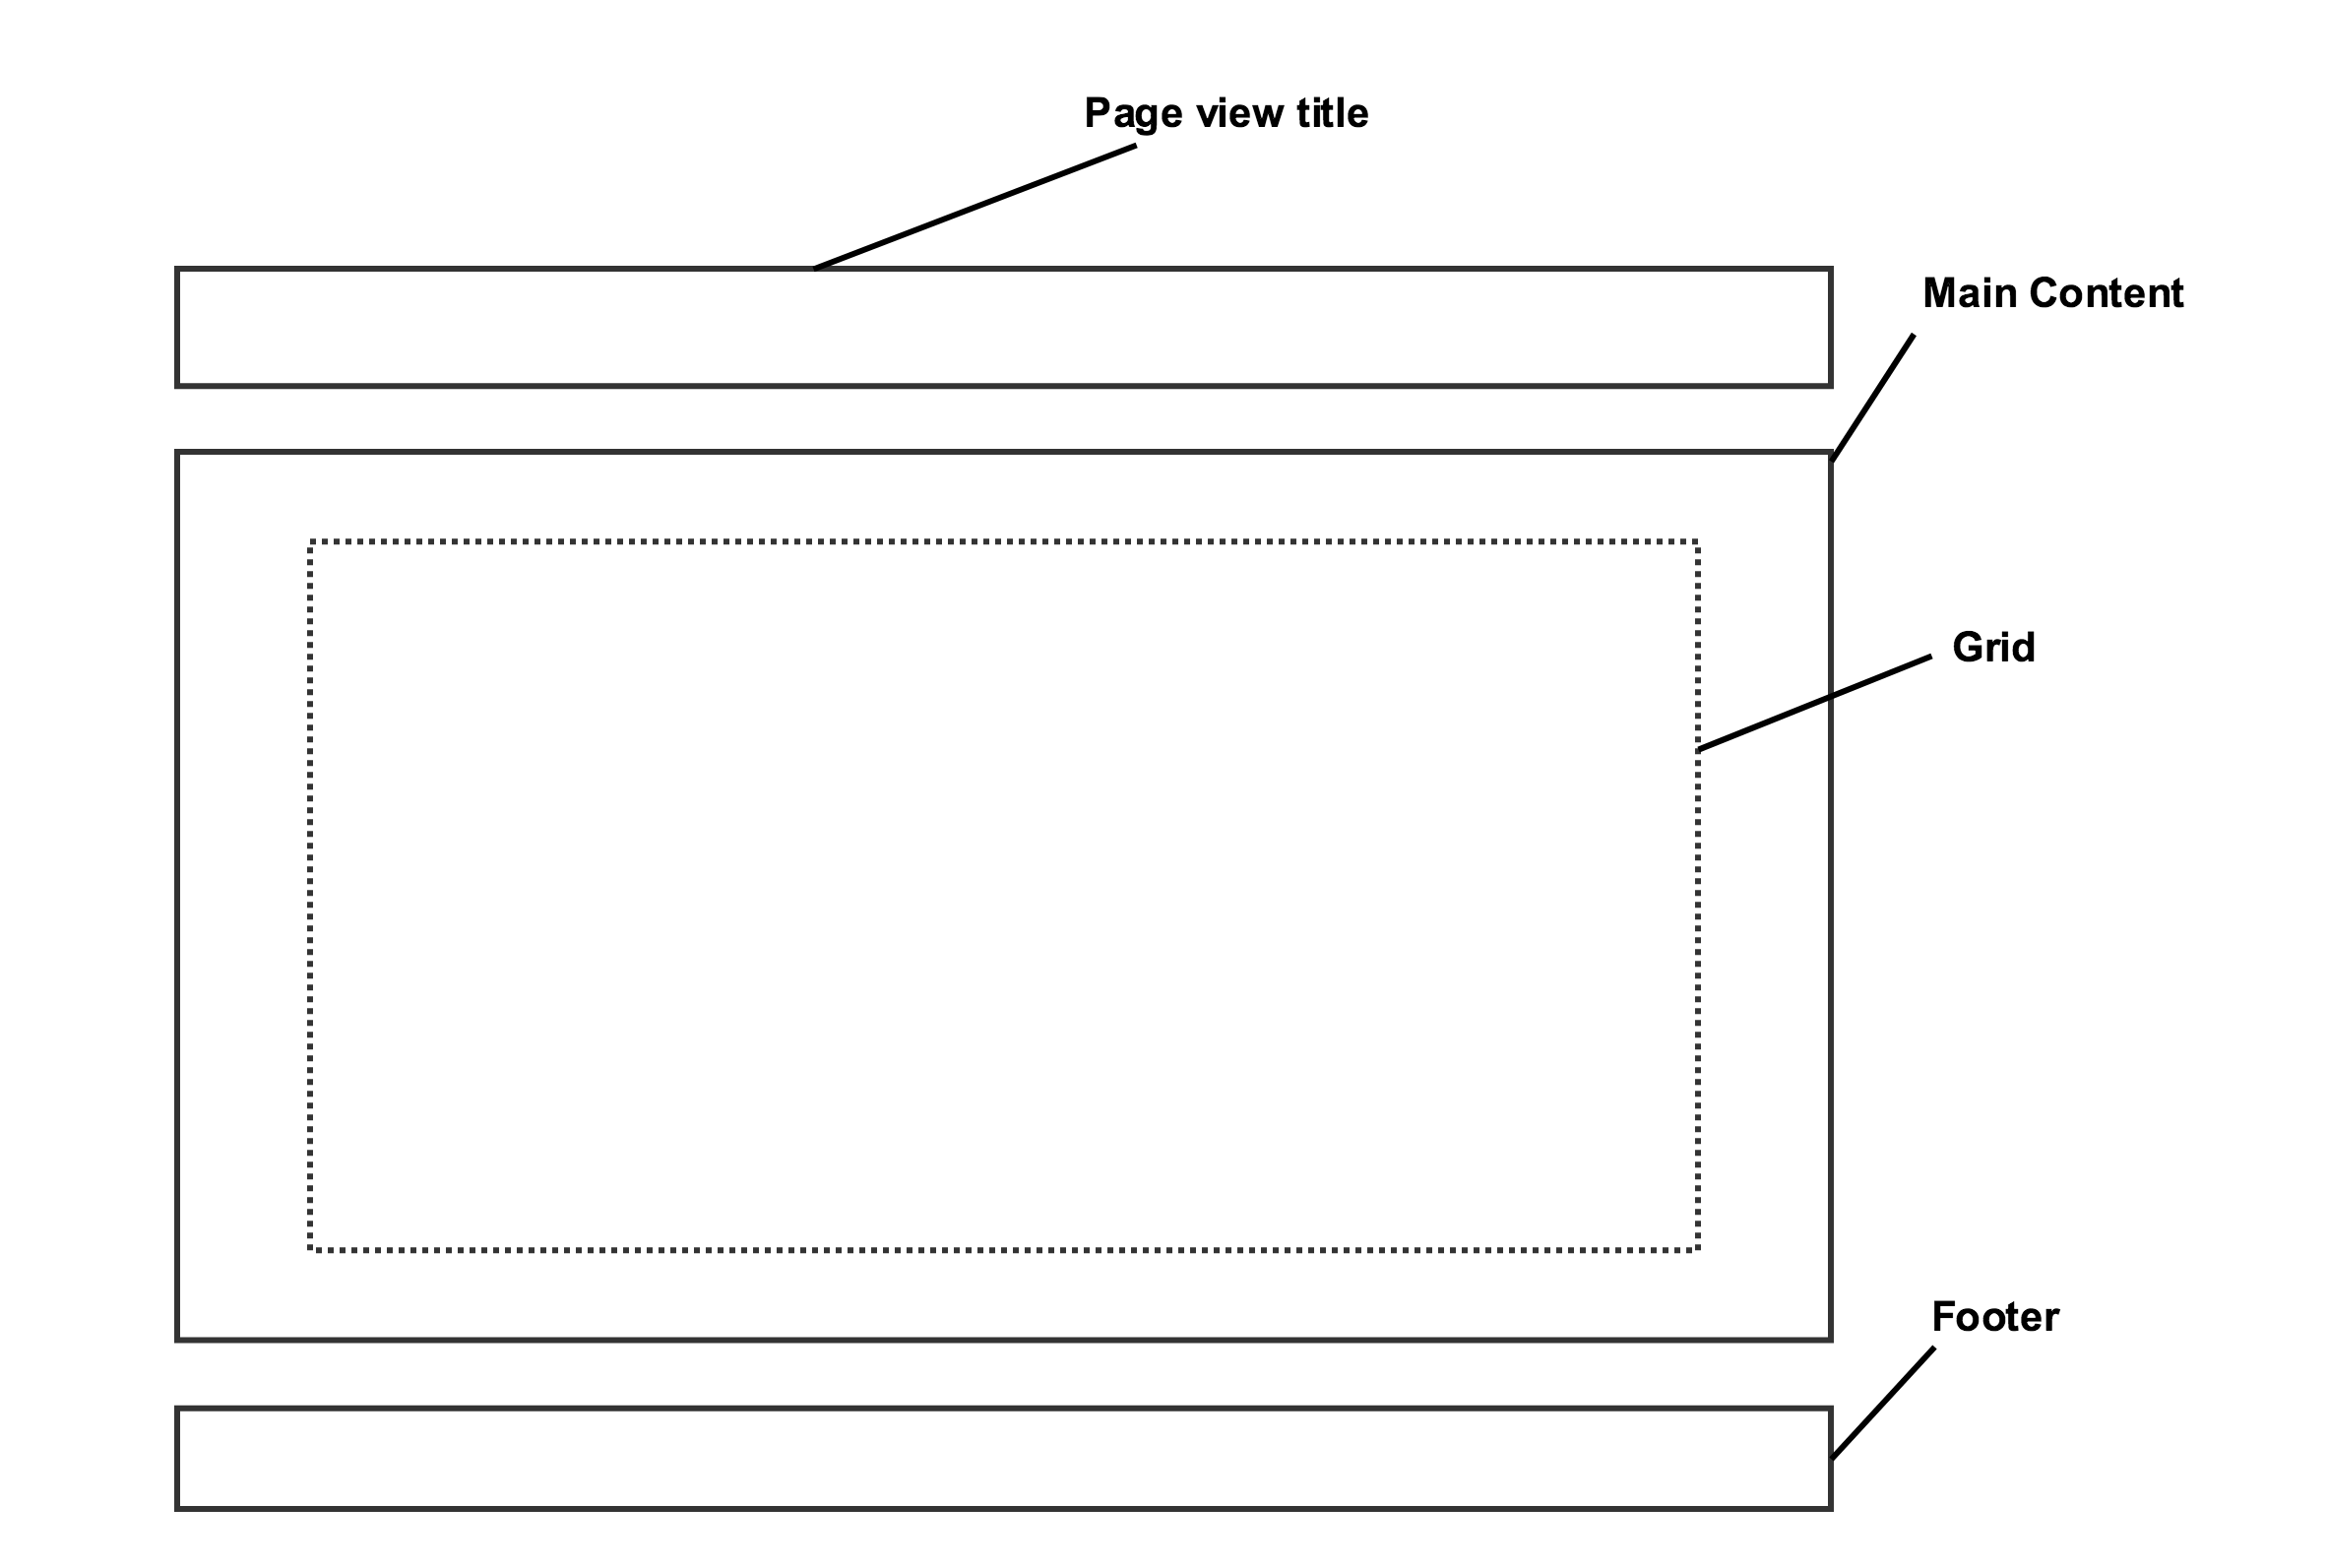
\includegraphics[width=\linewidth]{components/3/components/layout_basic.png}
  \caption{N2Sky Fundamental Layout}
  \label{fig:layout_basic}
\end{center}
\end{figure}

This layout applies styling like:
\begin{itemize}
\item Colors
\item Formatting
\item  Fonts
\item Positioning of elements and components
\end{itemize}



Fundamental Layout is a base layout which contains following elements:
\begin{itemize}
\item Page view title is a component with a caption and optionally an icon or push-to-action button
\item Main Content is centered component, which represent primary context. This component is always in focus of user and can contain one or more grid components.
\item Grid in basic layout represents positioning of elements, which can be displayed inside it. In basic layout in grid component is possible to add any elements. 
\item Footer is a component which goes across the whole application with a static data. Normally it is contacts and terms and conditions. 
\end{itemize}


\subsubsection{N2Sky Main Layout}\label{N2Sky Main Layout}

N2Sky Main Layout, which is shown in ``Fig.~\ref{fig:layout_main}'',  is extending N2Sky Fundamental Layout. Any changes in the basic layout will be automatically reflected in the main layout. Following components were added:

\begin{figure}[H]
\begin{center}
  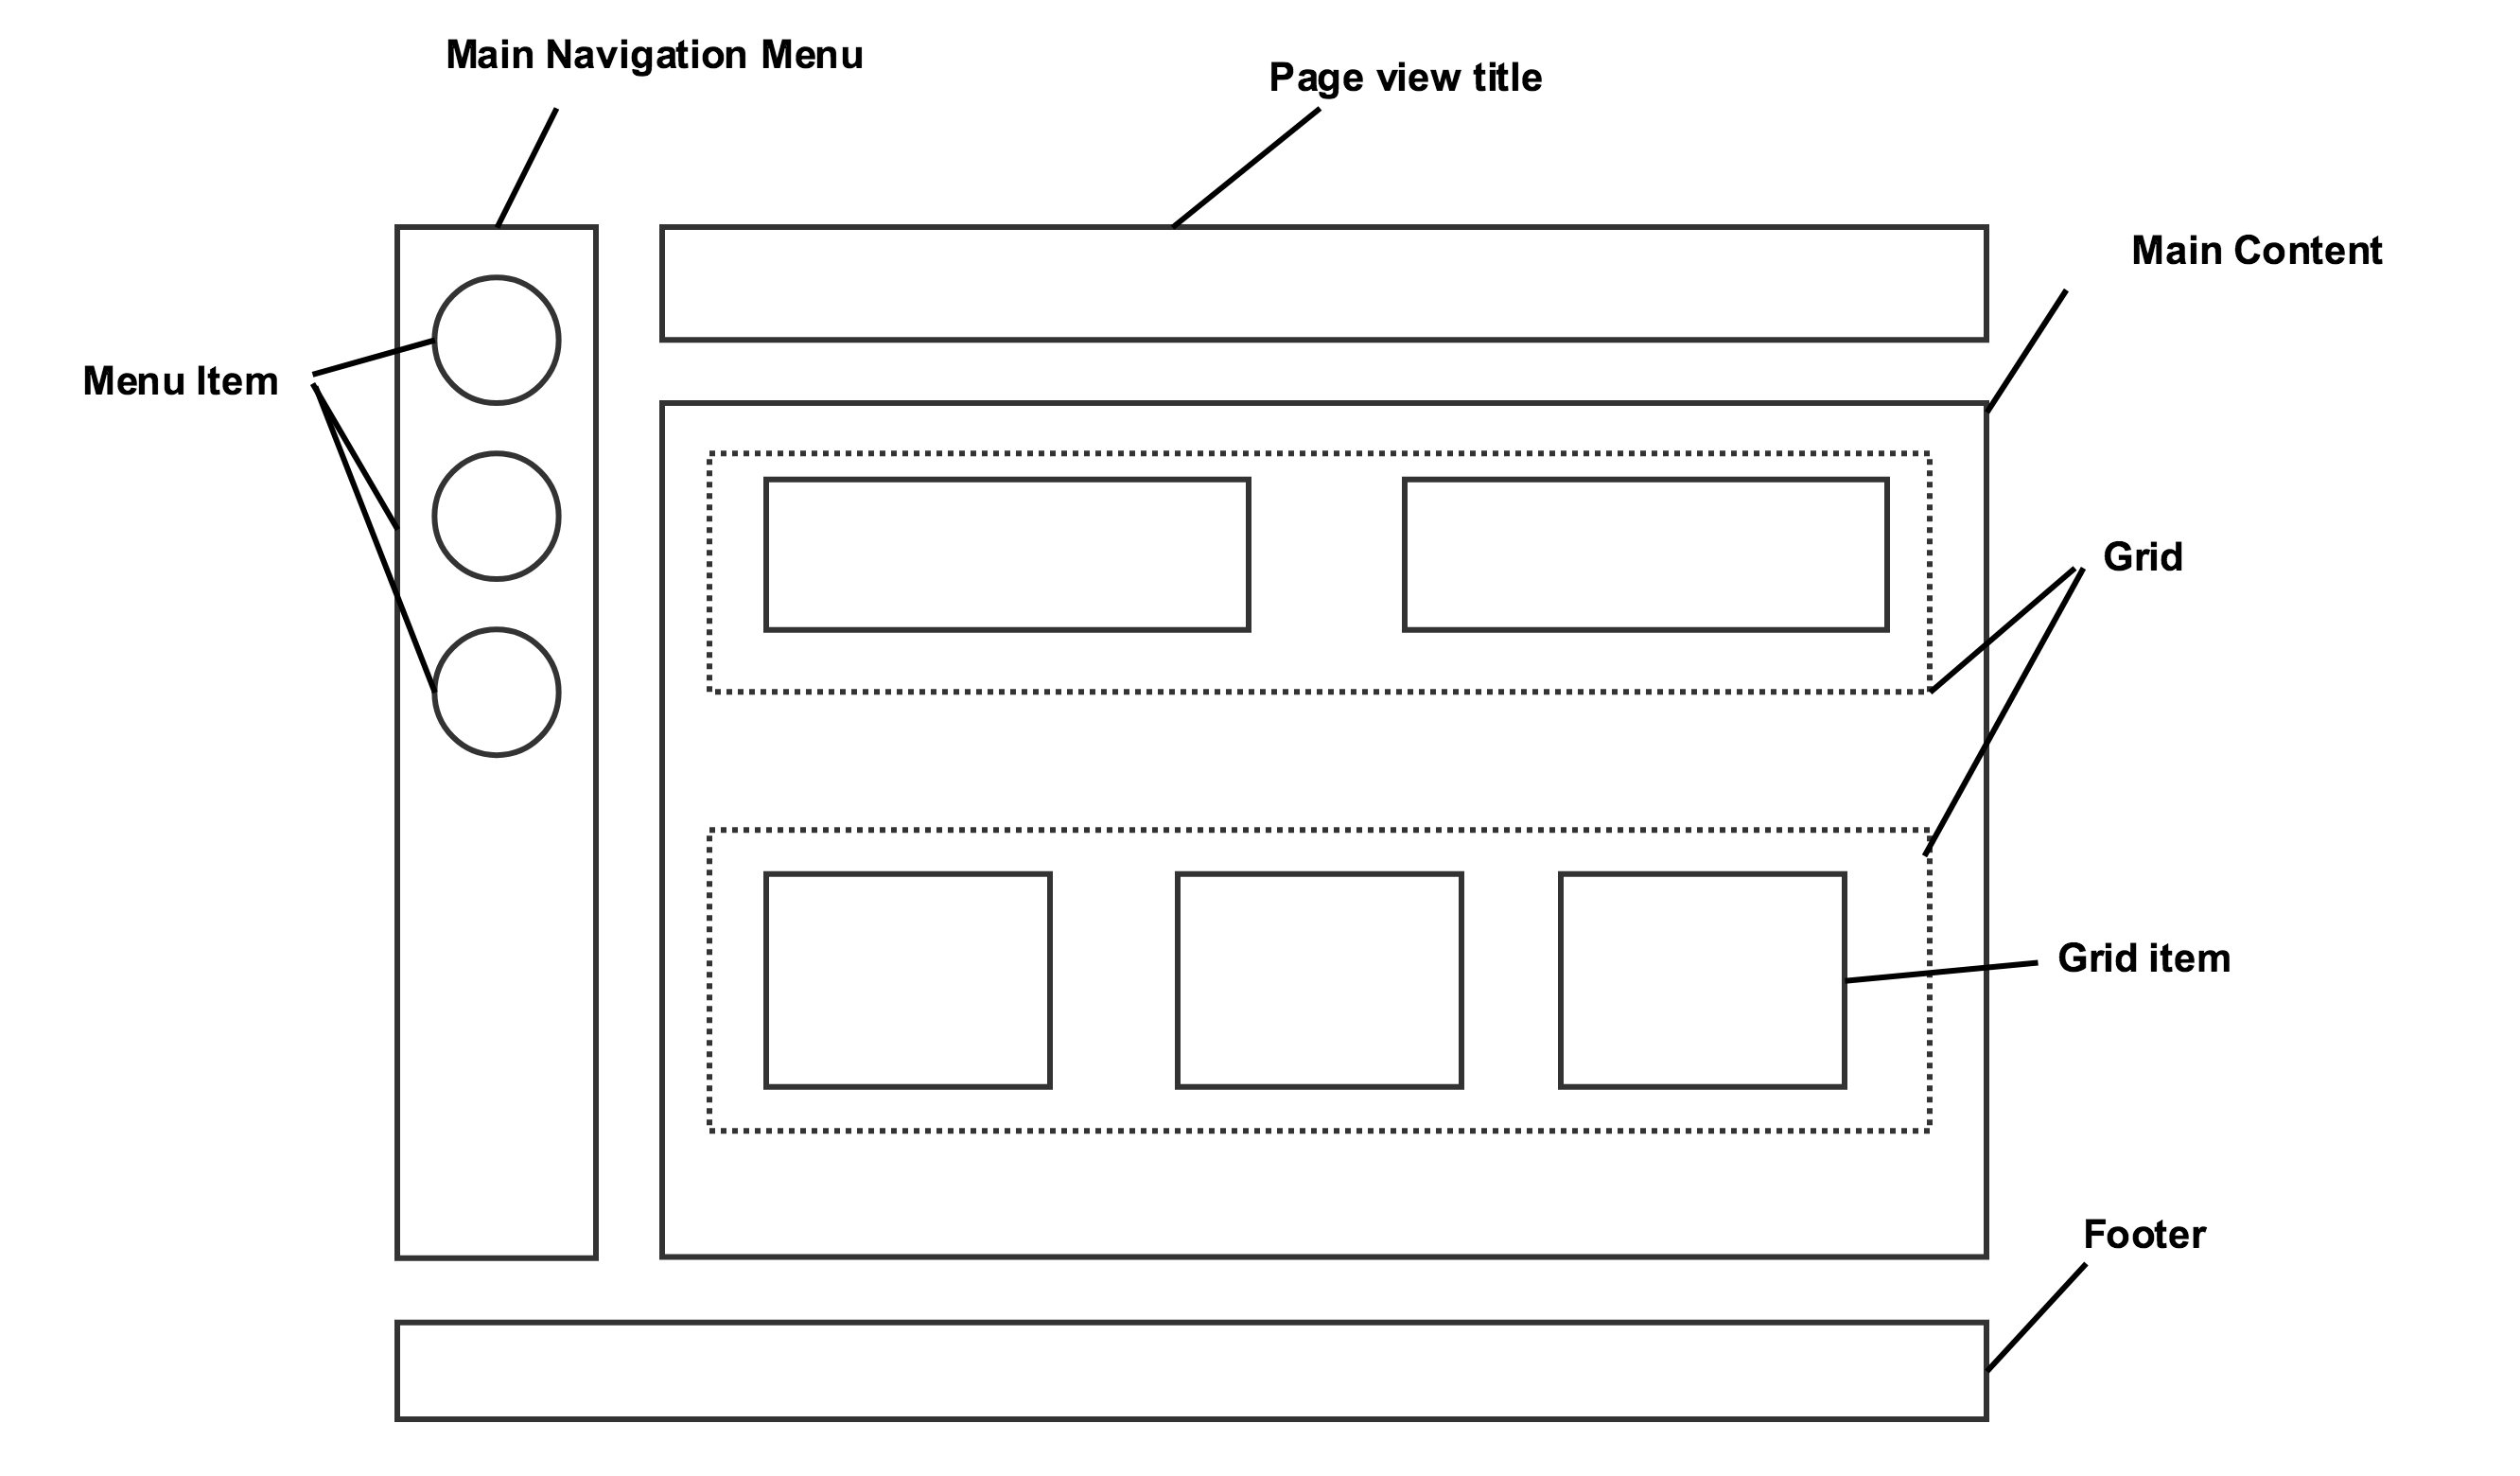
\includegraphics[width=\linewidth]{components/3/components/layout_main.png}
  \caption{N2Sky Main Layout}
  \label{fig:layout_main}
\end{center}
\end{figure}

\begin{itemize}
\item Main Navigation Menu, which displayed as a vertical bar. This component has two states: on mouse over it will be extended and menu items with a caption text and icon will appear, on mouse away from the component only menu items icon will be displayed. 
\item Menu items are icons with a captions components. Which items will be shown or hidden are depends on user permissions.
\item Grid items are blocking components, which can have multiple sizes but fixed within one grid. The context of grid item can be customized. 
\end{itemize}



\subsubsection{N2Sky Mobile Layout}\label{N2Sky Mobile Layout}

N2Sky supports mobile devices. For mobile devices, the mobile layout was developed as is shown in figure \ref{fig:layout_mobile}.

\begin{figure}[H]
\begin{center}
  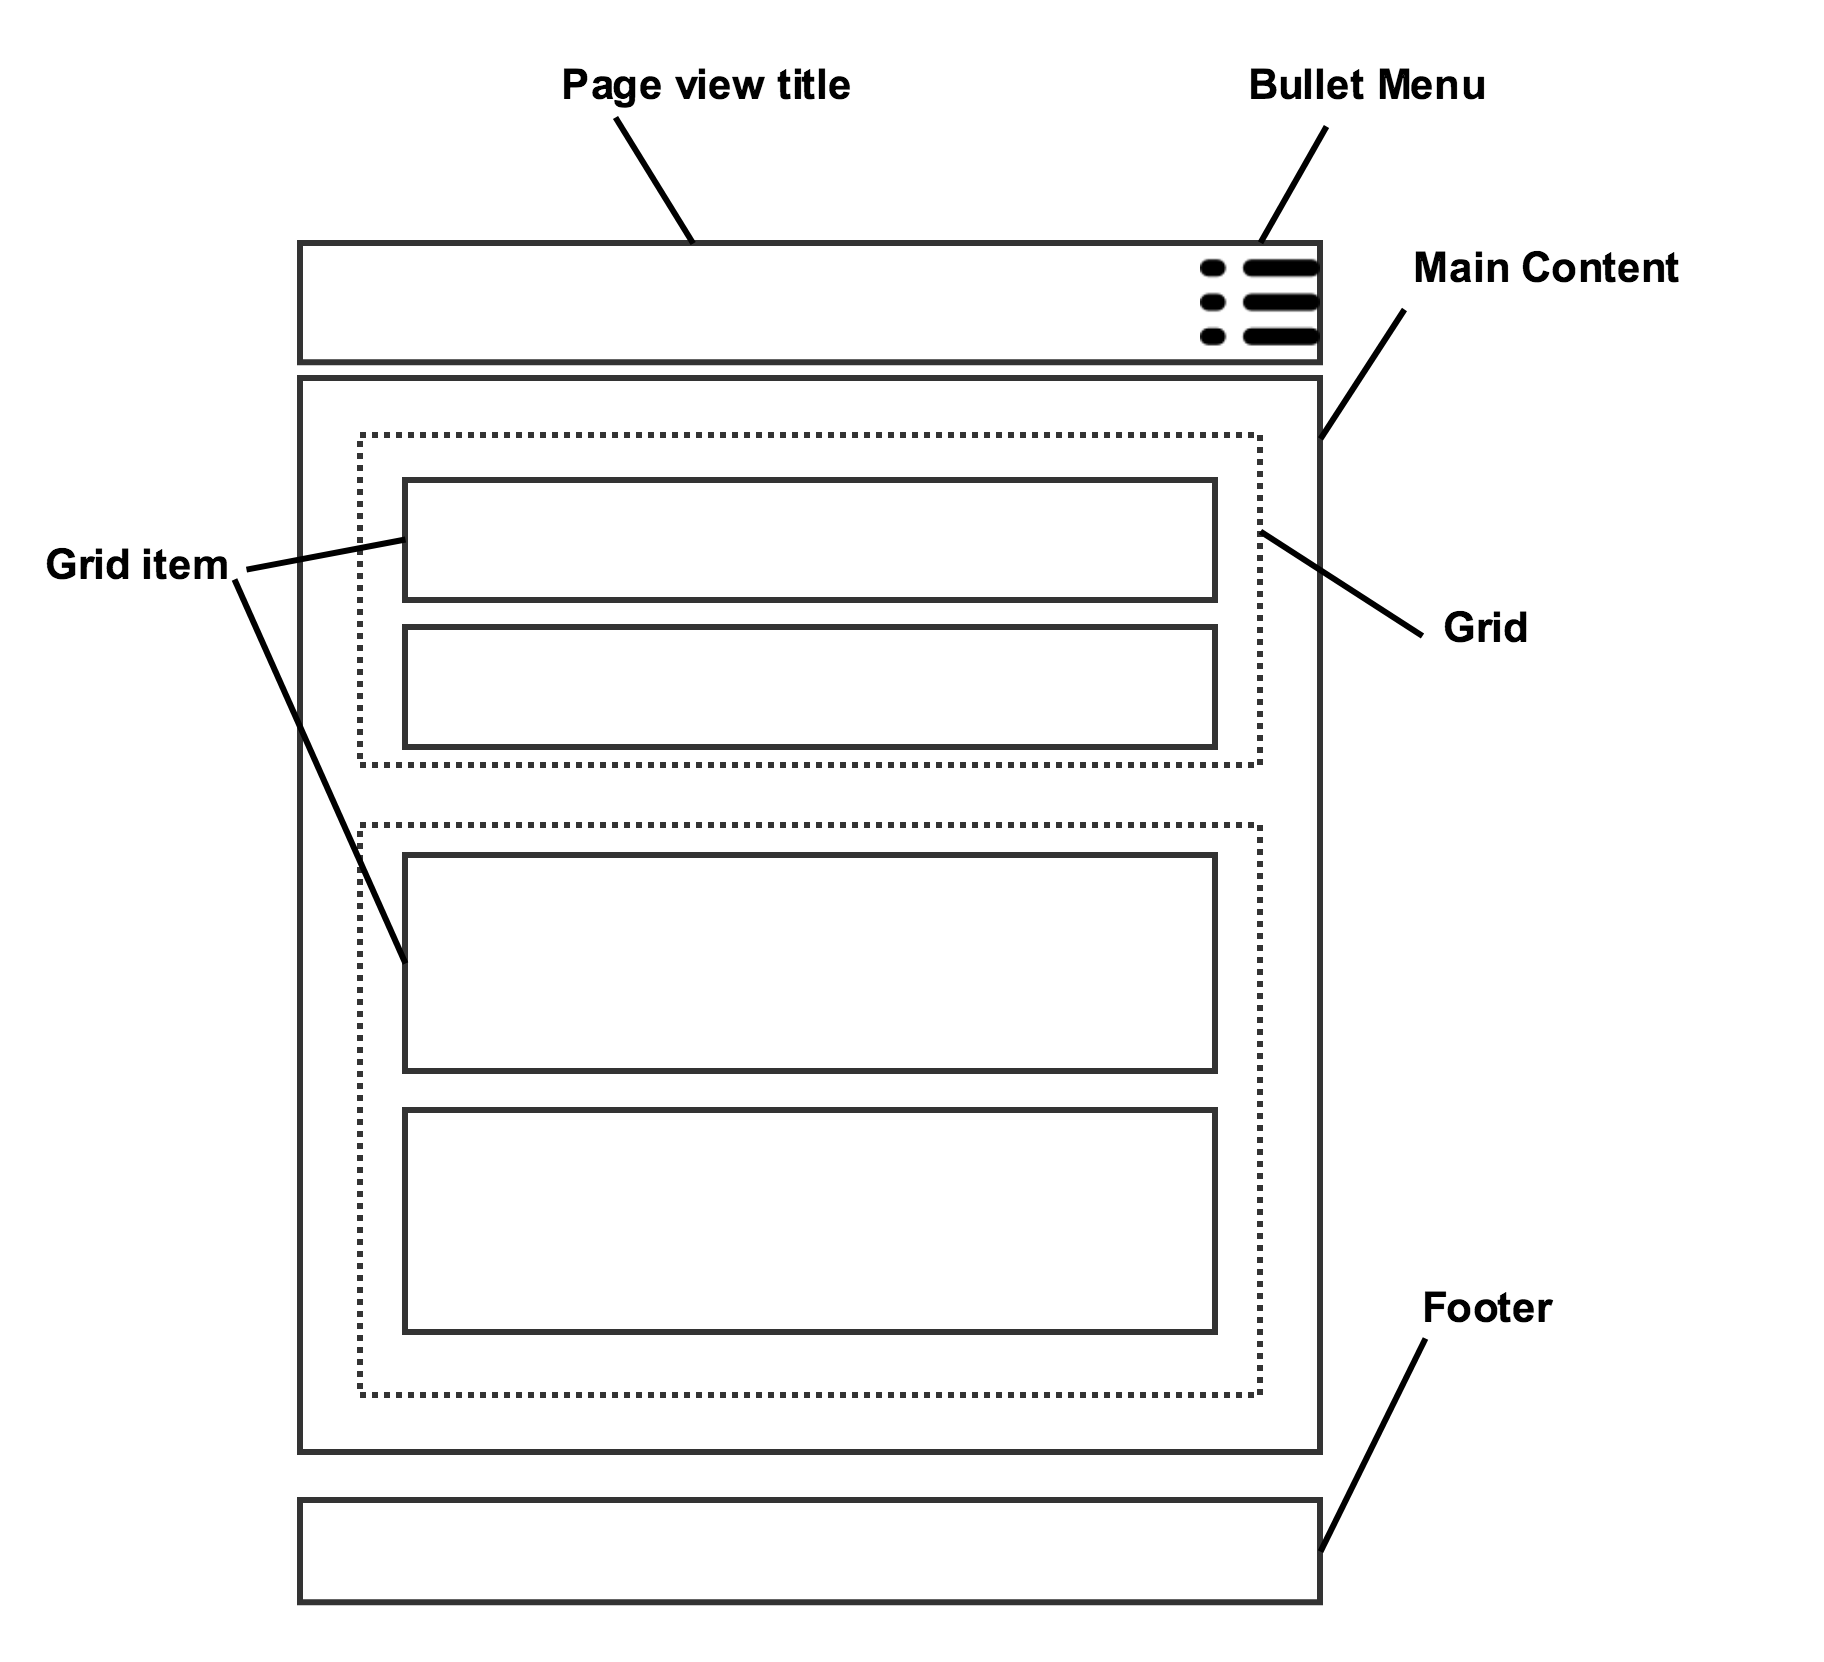
\includegraphics[width=\linewidth]{components/3/components/layout_mobile.png}
  \caption{N2Sky Mobile Layout}
  \label{fig:layout_mobile}
\end{center}
\end{figure}

All components context remain the same, but the positioning is changed. All grid items are vertically located and the width of grid items are the same as the device screen size. 

Additionally next to page view title component is Bullet Menu located. The normal desktop view is hidden and instead bullet menu perform the same functionality. On mouse click, the menu will appear as an overlay of the current view. 

\subsubsection{N2Sky Page Views}\label{N2Sky Page Views}

As it was mentioned in \autoref{Technology Stack} "Technology Stack", N2Sky frontend application developed on the ReactJS framework. Part of the ReactJS framework is React-Router, which contains all page views of the application and redirects it accordantly to URL path:

\begin{lstlisting}
<Provider store={store}>
	<Router history={browserHistory}>
		<Route path="/" component={Auth}/>
		<Route path="/signup" component={Reg}/>
		<Route component={AbstractDashboardLayout}>
			<Route path="/cloud" component={DashboardsOverview}/>
			<Route path="/user/profile" component={UserProfile}/>
			<Route path="/openstack" 
				component={OpenStackMainDashboard}/>
			<Route path="/openstack/project/:id"
				 component={OpenStackProjectDashboard}/>
			<Route path="/openstack/server/:projectid/:serverid" 
				component={ServerDetailsDashboard}/>
			<Route path="/openstack/vitrage/:templateId" 
				component={VitrageDetailsView}/>
			<Route path="/alert" component={AlertDashboard}/>
		</Route>
		<Route component={AbstractDashboardLayout}>
			<Route path="/n2sky" component={N2SkyDashboard}/>
			<Route path="/n2sky/available"
				 components={AvailableNetworksOverview}/>
			<Route path="/n2sky/models" 
				components={ModelsRepository}/>
			<Route path="/n2sky/paradigm/create/:projectid" 
				components={AddNNFromParadigm} readOnly={false}/>
			<Route path="/n2sky/paradigm/nn/:id" 
				components={AddNNFromParadigm} readOnly={true}/>
			<Route path="/n2sky/network/:id" 
				component={NetworkDetails}/>
			<Route path="/n2sky/network/:id/test/:model_id"
				 component={NetworkTestDetails}/>
			<Route path="/n2sky/project/:id"
				component={ProjectDashboard}/>
		</Route>
	</Router>
</Provider>
\end{lstlisting}

Every "Route" is a page view redirector and contains:
\begin{itemize}
\item Path, which responsible for URL redirection.
\item Component, which is a page view itself
\item Other props, which are optional
\end{itemize}

As it was mentioned in \autoref{Modular frontend application design} "Modular frontend application design", N2Sky contains two modules: Administration module and main application module. Both of this module sharing the same main application layout and having following page views: 
\begin{itemize}
\item \textbf{Administration Module:}
\begin{description}
\item[Cloud Dashboard View, path: "/cloud".] It is the main dashboard of Administration module, which contains overview dashlets of every modules component.
\item[OpenStack Dashboard View, path: "/openstack".] This view contains all information about OpenStack and the main control center of the OpenStack services.
\item[OpenStack Project, path: "/openstack/project/:id".] Route to the OpenStack project, which contains information about servers, flavours, images etc. of the particular project. In path "id" is the id of OpenStack project.
\item[Server Details View, path: "/openstack/server/:projectid/:serverid".] This view contains information about OpenStack instance. The URL path needs OpenStack project id and the id of the OpenStack instance. 
\item[Vitrage Details View, path: "/openstack/vitrage/:templateId".] Vitrage it a monitoring service of OpenStack and its instances. This view contains information about this service. The template id is required.
\item[Alert Management Dashboard View, path: "/alert".]  This view is a dashboard of Alert Management System. This view contains information about alerting rules and alerting events.
\end{description}

\item \textbf{Main Application Module:}
\begin{description}
\item[Authentication View, path: "/".] First page, which user sees, when he loading the application.  Authentication View contains login form.
\item[Registration View, path: "/signup".] Registration View contains registration form.
 \item[N2Sky Dashboard, path: "/n2sky".] Main Application Module view is the N2Sky Dashboard. This view contains information about logged in user projects, neural networks and trained models.  
\item[Available Networks View, path: "/n2sky/available".] This view is the neural network repository of the N2Sky. It is possible to copy available neural networks to own project.
\item[Models Repository View, path: "/n2sky/models".] The trained neural network are showed in this view. It is possible to copy published models to own project.
\item[Neural Network Create View, path: "/n2sky/paradigm/create/:projectid".] This view represents workflow of the creation of neural network from existing paradigm. The newly created neural network will be saved in user's project, hence this project id is required.  
\item[Neural Network Details View, path: "/n2sky/network/:id".] The details of the created neural network. It can be as well logged in user neural network or neural network from another user. User permissions show visibility level. The networks id is required. 
\item[Neural Network Test View, path: "/n2sky/network/:id/test/:model\_id".] From this view user can evaluate neural network this his own input parameters. Neural network id and trained model id are required. 
\item[Project Dashboard View, path: "/n2sky/project/:id".] This view shows the neural networks and models, which were created in particular project. The project id is required.
\end{description}


\end{itemize}






\subsubsection{N2Sky Dashboards}\label{N2Sky Dashboards}

The purpose of the dashboard is to embed business intelligent (BI) objects into the single page in order to make an overview of highlighted titles of BI objects \cite{dashboards_book}.

A dashboard has a structure layer upon its dashlets. It allows the user to manage layout and properties of dashlets. A dashboard is composed of dashlets. Every dashlet contains specific context and data. Dashboard defines: 
\begin{itemize}
\item Dashlets to be displayed
\item The layout of dashboard and positioning of its dashlets
\item The common context of particular dashlets
\end{itemize}


\begin{figure}[H]
\begin{center}
  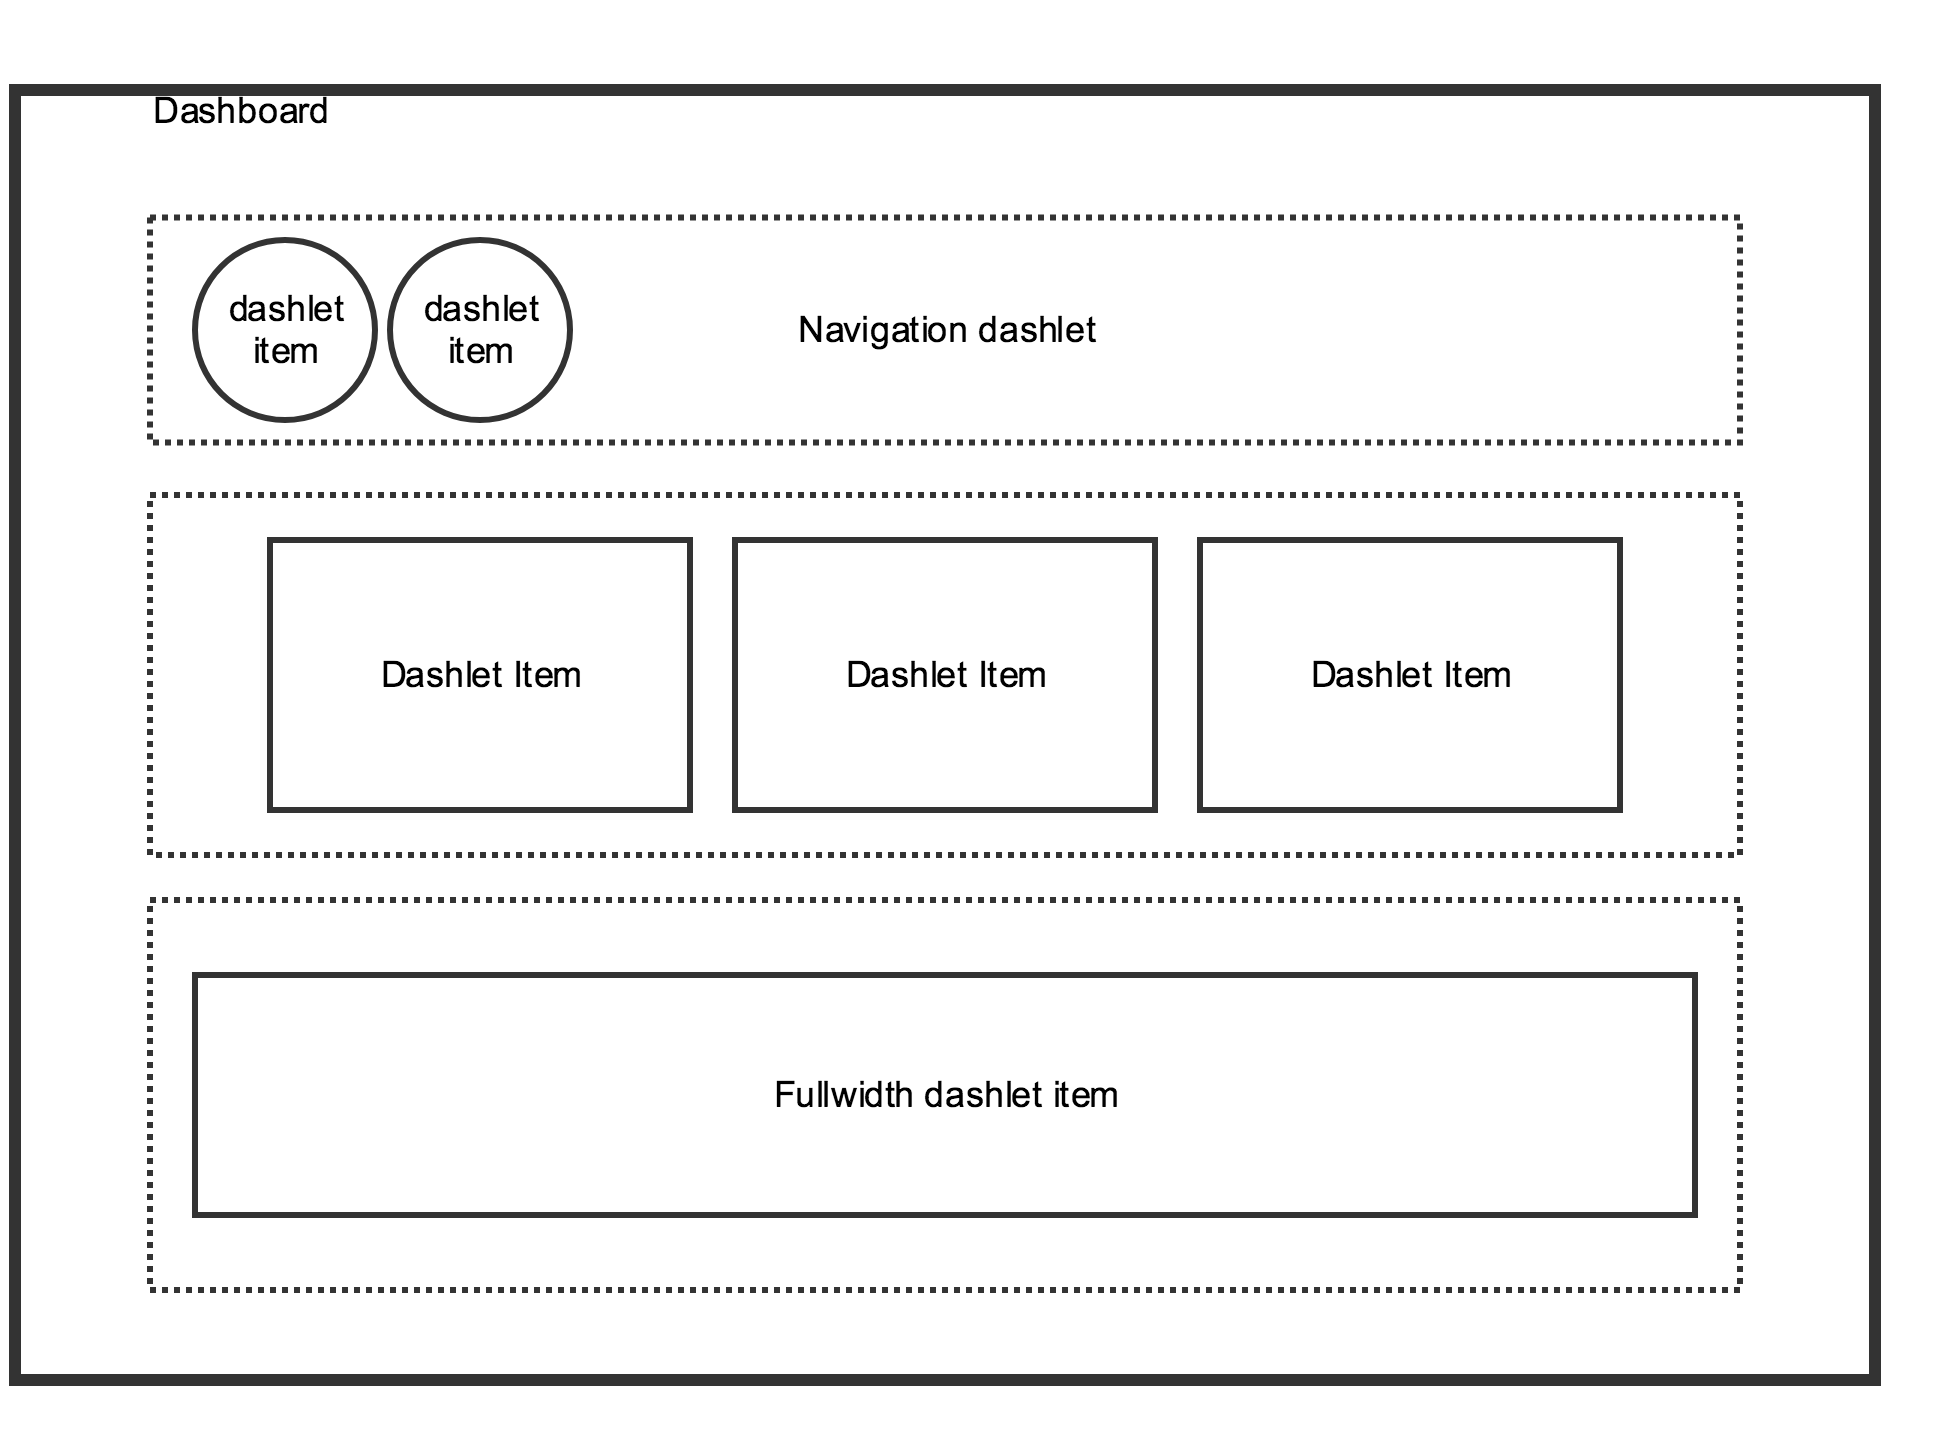
\includegraphics[width=\linewidth]{components/3/components/dashboard_template.png}
  \caption{N2Sky Dashboard template}
  \label{fig:dashboard_template}
\end{center}
\end{figure}

In the figure \ref{fig:dashboard_template} is shown the typical N2Sky dashboard template. A dashboard in N2Sky has a grid structure. Every dashlet has one or more items. Every item can contain any UI component, but it has to be feet into assigned dashlet without overlays. 



\subsubsection{Responsive design}\label{Responsive design}

Since N2Sky is cross-platform application it has to support multiple screen resolutions as well as readability and usability. 

Considering readability first of all the typography has to be mentioned. During development of N2Sky to find the fonts, which will be displayed same and will be readable across multiple devices was a challenge. The typeface \cite{wiki:typeface} properties like latter spacing, width, weight etc were adjusted multiple times. The common problem was to audit how typeface represents on mobile devices and desktop computers \cite{responsive_book}. Even such a standard fonts like "Arial" and "Times New Roman" were looking unreadable on mobile devices as it is shown in figure \ref{fig:typo}.

\begin{figure}[htbp]
\begin{center}
  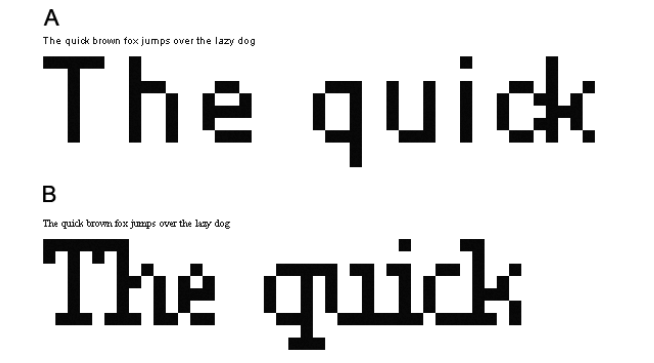
\includegraphics[scale=0.5]{components/3/components/typo.png}
  \caption{Difference between sans-serif font Arial (A) and the browser serif font Times New Roman (B) }
  \label{fig:typo}
\end{center}
\end{figure}

The expansion of cross-platform applications brought some freedom to developers and designers. Today is possible to develop an application simultaneously for mobile devices, desktop computers, and web browsers. The problem comes, when the mobile and tablet devices manufacturers started to produce devices with different resolutions. Today versioning of mobile screen resolution came over 1000 devices, but N2Sky was concentrating only on major market players as it is shown in figure \ref{fig:screen} \cite{mobile_resolution}.

\begin{figure}[htbp]
\begin{center}
  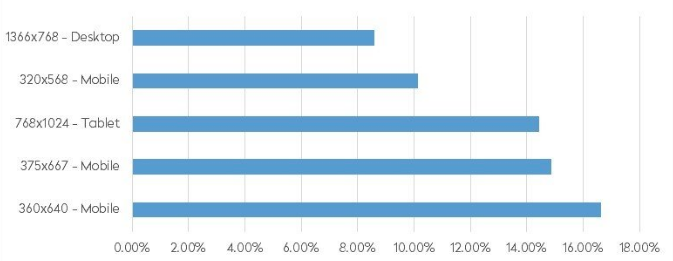
\includegraphics[scale=0.65]{components/3/components/screen.png}
  \caption{Average screen resolution of mobile, tablet and desktop devices on 2017}
  \label{fig:screen}
\end{center}
\end{figure}

N2Sky is focused on mobile and tablet devices because it is an extensive trend nowadays. 

\subsubsection{User Interface Elements}\label{User Interface Elements}

It is possible to divide all UI elements into groups \cite{intelligent_support}:

\begin{description}
\item[Input Controls.] Input controls determine user input action. Input actions are keyboard typing or mouse clicking.  Following UI elements are the part of input controls: 
\begin{itemize}
\item Checkboxes
\item Radio buttons 
\item Dropdown Lists
\item List boxes
\item Buttons
\item Toggles
\item Text fields
\item Date field
\end{itemize}
\item[Navigational Components.] Navigation between page views. Navigational components include also some particular request from and to the user. Following UI elements are the parts of navigational components:
\begin{itemize}
\item Breadcrumb 
\item Slider
\item Search field
\item Pagination
\item Slider
\item Tags
\item Icons
\end{itemize}
\item[Informational Components.] These components are the addition to workflows. It can help the user to perform some actions or they can inform the user, that the action will occur or already occurred. Informational Components contains following UI elements:
\begin{itemize}
\item Tooltips
\item Icons
\item Progress bar
\item Notifications
\item Message boxes
\item Modal windows
\end{itemize}
\item[Containers.] Containers are components, which are hiding additional information or not focused information, where the user needs to perform the action in order to see it.   
\begin{itemize}
\item Accordion
\item Semi-hidden elements
\end{itemize}
\end{description}

\subsubsection{UI Elements in N2Sky}\label{UI Elements in N2Sky}

N2Sky supports almost all common web user interface elements. Every element was developed in order to be reusable. Since N2Sky supports responsive design, the UI elements should also be responsive. Every UI element is absolute customised. Following UI elements were created:

\begin{description}
\item[Accordion]  Accordion is a list of items, which is accessible on mouse click. In N2Sky accordion works more like a modal window. With this kind of functionality other data, which surround accordion will not be stretched or squeezed but will appear on top of elements as it is shown in figure \ref{fig:accordion}: 

\begin{figure}[htbp]
\begin{center}
  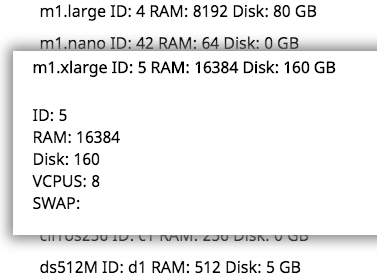
\includegraphics[scale=0.75]{components/3/components/accordion.png}
  \caption{Customised N2Sky accordion UI element}
  \label{fig:accordion}
\end{center}
\end{figure}

\item[Buttons.] Idea behind was to make buttons more interactive and understandable to use as it is displayed in \ref{fig:button_inactive}. Buttons contain caption and icon in SVG format in order to support high quality image in all devices.

Buttons are using on hover animation. When mouse over the button, then button icon slide to the middle to show that action can be performed as it is shown in figure \ref{fig:button_active}. 

\begin{figure}[htbp]
\begin{center}
  
\includegraphics[scale=0.55]{components/3/components/button_inactive.png}
  \caption{Customised N2Sky button UI element}
  \label{fig:button_inactive}
\end{center}
\end{figure}


\begin{figure}[htbp]
\begin{center}
  
\includegraphics[scale=0.55]{components/3/components/button_active.png}
  \caption{Customised N2Sky button UI element animation}
  \label{fig:button_active}
\end{center}
\end{figure}

\item[Icons.] In N2Sky all icons are in Scalable Vector Graphics (SVG) format. With SVG the icons do not lose quality in any device \cite{Cagle2005}. Since it is a vector graphic it easy to edit an icon with programming language code. N2Sky Logo, which is represented in figure \ref{fig:logo},  is also made in SVG format. 

\begin{figure}[htbp]
\begin{center}
  
\includegraphics[scale=0.55]{components/3/components/logo.png}
  \caption{Customised N2Sky logo in SVG format}
  \label{fig:logo}
\end{center}
\end{figure}

Is it possible to import code in some graphical vector editor in order change color, path (vector graphic itself), metadata etc. Following code demonstrate N2Sky Logo in SVG format. The whole vector path was shortened.

\begin{lstlisting}
<?xml version="1.0" standalone="no"?>
<!DOCTYPE svg PUBLIC "-//W3C//DTD SVG 20010904//EN"
        "http://www.w3.org/TR/2001/REC-SVG-20010904/DTD/svg10.dtd">
<svg version="1.0" xmlns="http://www.w3.org/2000/svg"
     width="266.000000pt" height="267pt" viewBox="0 0 266 267"
     preserveAspectRatio="xMidYMid meet">
    <metadata>
        N2Sky Logo. 2018
    </metadata>
    <g transform="translate(0.000000,267.000000) scale(0.100000,-0.100000)"
       fill="#6b6b6b" stroke="none">
        <path d="M1302 2638 c-9 -9 -12 -83 -12 -270 0 -245 -1 -259
-37 -26 -170 21 -63 23 -132 46 -152 52 -23 7 -38 17 -38 27 1
80 222 90 255 87 284 -2 23 -9 32 -25 34 -27 4 -46 -23 -72 -106 
-77 -34 -95 -8 -18 -22 -51 -32 -74 -10 -24 -21 -43 -25 -43 -5 0 -30 
76 -76 118 -100 136 -128 92 -12 -20 -10 -26 101 -219 35 -60 109 

...

-18 74 -40 36 -22 67 -40 70 -40 11 0 253 -152 269 -169 11 -12 15 -27 12 
-36 26 -103 -14 -32 -19 -60 -35 -62 -35 -3 0 -34 -18 -70 -40 -36 -22 -68
-40 -70 -40 -3 0 -22 -11 -43 -23 -142 -90 -172 -96 -201 -39 -20 40 -47 168
-55 268 l-5 61 122 22 c67 13 156 30 197 38 85 16 106 30 95 63 -7 21 -11 22
-69 16 -33 -4 -88 -10 -121 -15 -178 -26 -178 -26 -170 -1 4 13 21 46 37 74
57 100 63 116 52 134 -6 9 -22 17 -34 17 -24 0 -47 -33 -130 -180 -75 -132
-74 -130 -61 -206 6 -38 16 -102 21 -141 6 -40 15 -98 20 -129 6 -30 10 -72
10 -93 l0 -38 -162 4 c-151 3 -167 5 -212 28 -82 43 -86 57 -86 320 l0 226 38
34 c21 19 53 47 72 61 19 14 49 39 67 55 17 16 54 47 82 69 60 49 79 79 65
103 -18 28 -47 25 -84 -10 -20 -18 -52 -45 -72 -60 -20 -15 -42 -34 -50 -41
-23 -23 -92 -67 -105 -67 -10 0 -13 27 -13 104 0 57 -3 111 -6 120 -7 19 -45
21 -62 4z"/>
    </g>
</svg>
\end{lstlisting}

\item[Notification messages.] Notification messages are the part of information component. In N2Sky used two types of notification messages: 
\begin{itemize}
\item Waring message, which tells, that something goes wrong as it shown in ``Fig.~\ref{fig:notif_warning}''. It can be an error in the application as well as user workflow error. 
\item Informational message that gives information about the event which will occur or already occurred as it shown in ``Fig.~\ref{fig:notif_info}''.
\end{itemize}


\begin{figure}[htbp]
\begin{center}
  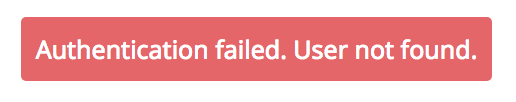
\includegraphics[scale=0.65]{components/3/components/notif_warning.png}
  \caption{Customised N2Sky warning message UI element}
  \label{fig:notif_warning}
\end{center}
\end{figure}

\begin{figure}[htbp]
\begin{center}
  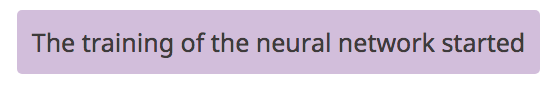
\includegraphics[scale=0.65]{components/3/components/notif_info.png}
  \caption{Customised N2Sky informational message UI element}
  \label{fig:notif_info}
\end{center}
\end{figure}

\item[Navigation.] In N2Sky user can navigate to another one page or change part of the page view via tabs, navigation buttons, and menus. 
Navigation elements are bind to the group of element or UI components. Following navigation component which is shown in ``Fig.~\ref{fig:nav}'', contains navigation elements as well functional icon. 
\end{description}

\begin{figure}[htbp]
\begin{center}
  
\includegraphics[scale=0.65]{components/3/components/nav.png}
  \caption{Customised N2Sky navigation UI element}
  \label{fig:nav}
\end{center}
\end{figure}

Navigation bars can contain tabs, buttons, icons and non-functional text. ``Fig.~\ref{fig:nav_bar}'' shows navigation bar an custom table. 

\begin{figure}[htbp]
\begin{center}
  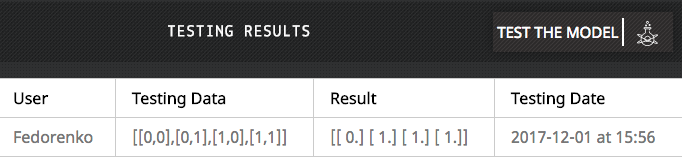
\includegraphics[scale=0.65]{components/3/components/nav_bar.png}
  \caption{Customised N2Sky navigation bar with a table}
  \label{fig:nav_bar}
\end{center}
\end{figure}

\subsubsection{UI Components in N2Sky}\label{UI Components in N2Sky}

Groups of UI elements form UI components. Components, like elements, are also fully reusable, the only context of components is changing. Following custom UI components were developed in N2Sky: 

\begin{description}
\item[Grid Item Component.] Grid in N2Sky is responsive. It can change positions and size of grid items like it shown in ``Fig.~\ref{fig:grid_item}''. 

\begin{figure}[htbp]
\begin{center}
  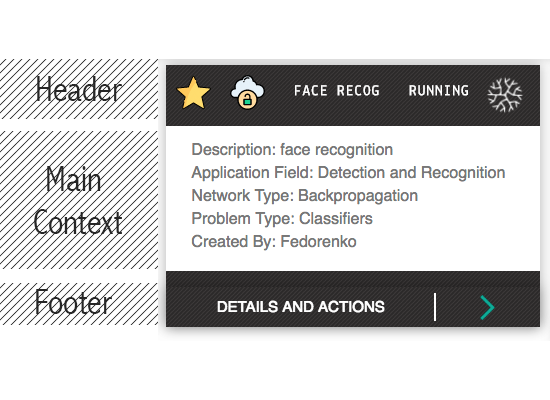
\includegraphics[scale=0.65]{components/3/components/grid_item.png}
  \caption{Responsive N2Sky Grid Item UI comonent}
  \label{fig:grid_item}
\end{center}
\end{figure}


Grid item contains following UI element: 
\begin{description}
\item[Header. ] Header is the first component on which the user focuses, that is why it should be short but highlighted. Following UI elements are included: 
\begin{itemize}
\item Functional icons-buttons on the left side (optional)
\item Title of grid item (mandatory)
\item  Non-functional icons (optional)
\end{itemize}
\item[Main context. ] Component, which contains context information. This component can be fully customized. It is possible to put there the list of items, plain text or even image.
 \item[Footer. ] Footer is an optional element and contains only button UI element. 
\end{description}

\item[Main navigation menu.] Every N2Sky view use main navigation menu, namely, the menu is injected in an abstract view, which is extended by all other view components. The menu has menu items, which contain caption and an icon. As it was mentioned before, N2Sky has two modules: administration module and main application module. Both modules are represented in menu and menu items visibility depending on logged-in user permission. 
Menu for arbitrary user is shown in figure \ref{fig:menu_user}  and has following menu items:

\begin{itemize}
\item Profile 
\item N2Sky Dashboard
\item Available neural networks
\item Models repository
\end{itemize}

 
 \begin{figure}[htbp]
\begin{center}
  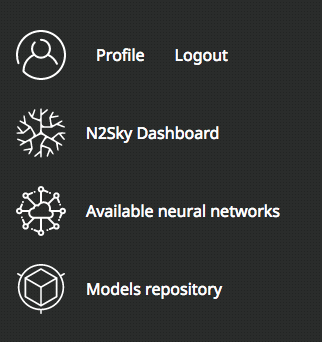
\includegraphics[scale=0.65]{components/3/components/menu_user.png}
  \caption{N2Sky Main Navigation Menu for arbitrary user}
  \label{fig:menu_user}
\end{center}
\end{figure}

If end-user is a system administrator, he can see additional menu form administration module as is demonstrated in ``Fig.~\ref{fig:menu_admin}'. This menu contains dropdown submenus: 

\begin{itemize}
\item OpenStack Dashboard
\item Cloudify Dashboard
\item Alert System
\item Dashboards Settings
\end{itemize}


 \begin{figure}[htbp]
\begin{center}
  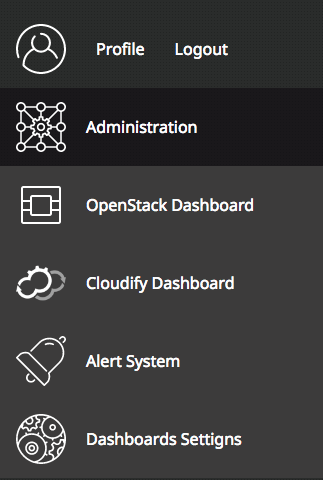
\includegraphics[scale=0.65]{components/3/components/menu_admin.png}
  \caption{N2Sky Main Navigation Menu for system administrator}
  \label{fig:menu_admin}
\end{center}
\end{figure}

\item[Modal windows.] N2Sky use modal windows almost in every view as it is shown in figure \ref{fig:modal}. Modals are responsive and touch screen friendly. It has 3 elements:
\begin{itemize}
\item Title (mandatory)
\item Context (mandatory)
\item Submit button (optional)
\end{itemize}

 \begin{figure}[H]
\begin{center}
  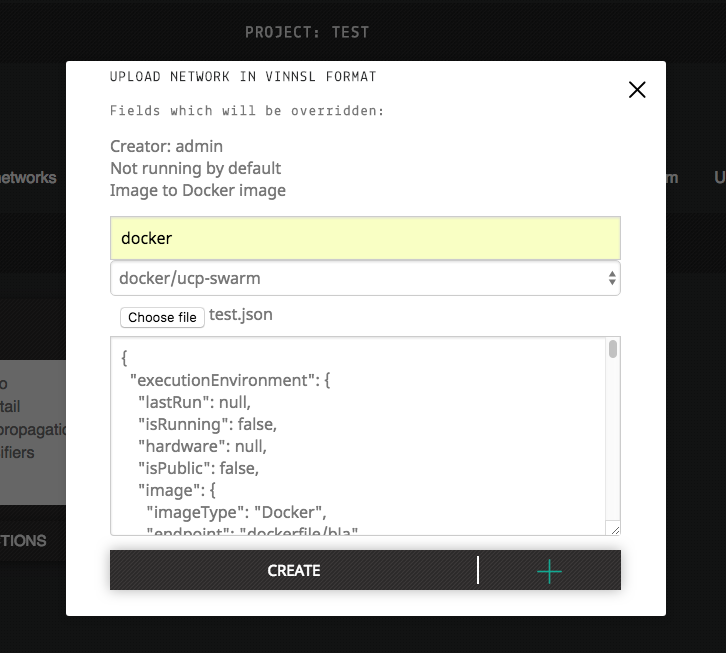
\includegraphics[scale=0.5]{components/3/components/modal.png}
  \caption{N2Sky Modal Window UI component}
  \label{fig:modal}
\end{center}
\end{figure}

Modals can be used to represent form as well for informational purposes. When modal is open the background is dunned in order to focus the user on modal context. The modal context itself can be fully custom. It is possible to put any UI element in context.



\end{description}



\subsection{N2Sky Services}\label{N2Sky Services}

 N2Sky implements the microservices architecture. It has 3 main web services as it is shown in figure \ref{fig:newarch}:
 
\begin{itemize}
\item User Management Web Service
\item Model Repository Web Service
\item Cloud management Web Service
\end{itemize}

Every web service uses other services which are not exposed to the public. It was made in order to support application encapsulation. Encapsulation of web application helps to prevent security issue. One of the crucial crucial processes in N2Sky is the neural network training. This process takes almost all resources of the environment, that is why it is not exposed. Such a process can be triggered only by web service, which can be blocked if the environment is overloaded.

Consider the following web services in details and which processes and services they are encapsulated:  


\subsubsection{User Management Web Service.}\label{User Management Web Service}   This web service responsible for permissions and user management and it has its own database. The user can authorize in the system and get a session token. Every token is a unique collection of numbers and Latin letters. The token is assigned to the authorized user and will be saved until the user is active. If the user is not active in the next 3 hours, the session token will disappear. If the user still has an active browser session, the authorization token will be revalidated. If user trying to make some illegal request or behave too active, the authorization token will be revoked and the system administrator will be notified of this incident. 

Every user encapsulates permission level. There two different types of permissions:
\begin{itemize}
\item Administrator permission. It means, that the user has full granted permission throw entire application.
\item Regular permission. The user has access only for his own as well as publicly available resources.  
\end{itemize}

 \begin{figure}[H]
\begin{center}
  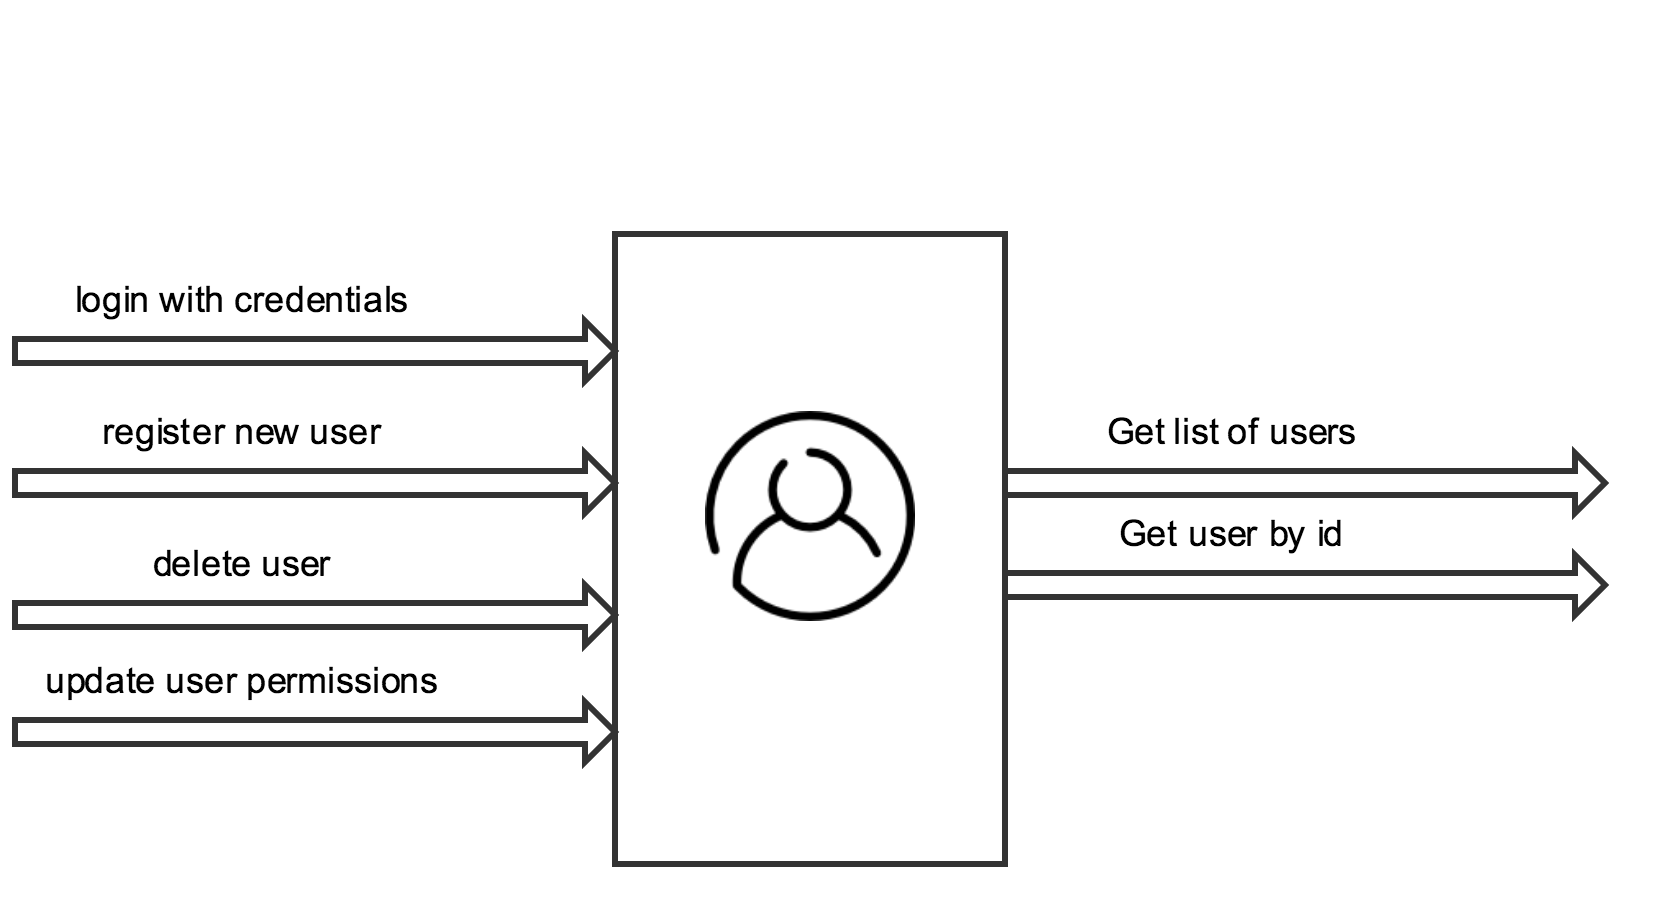
\includegraphics[width=\linewidth]{components/3/components/user_serivice.png}
  \caption{N2Sky User Management Web Service}
  \label{fig:user_serivice}
\end{center}
\end{figure}

As is shown in ``Fig.~\ref{fig:user_serivice}'' User Management Web Service has following accessible services:

\begin{itemize}
\item Login with credentials
\item Register a new user 
\item Delete user
\item Update user permissions
\item Get list of users
\item Get user by user ID
\end{itemize}
 
 Detailed information about web service API and API documentation is written in \autoref{API Documentation}

\subsubsection{Model Repository Web Service.}\label{Model Repository Web Service}  Model Repository Web Service is the core service of N2Sky. The authorized user can create a new project, add their neural network from chose paradigm or deploy own one. Every newly created project is assigned to one user and can not be shared, the only system administrator can look up into other users projects. This functionality also limited by User Management Web Service. 

Using this service user can create a neural network from proposed paradigms as well as upload his own neural network in ViNNSL format \cite{Beran2008}. This functionality exposed via service so that every user can use it either from N2Sky web portal or via HTTP request directly on web service.

\begin{figure}[H]
\begin{center}
  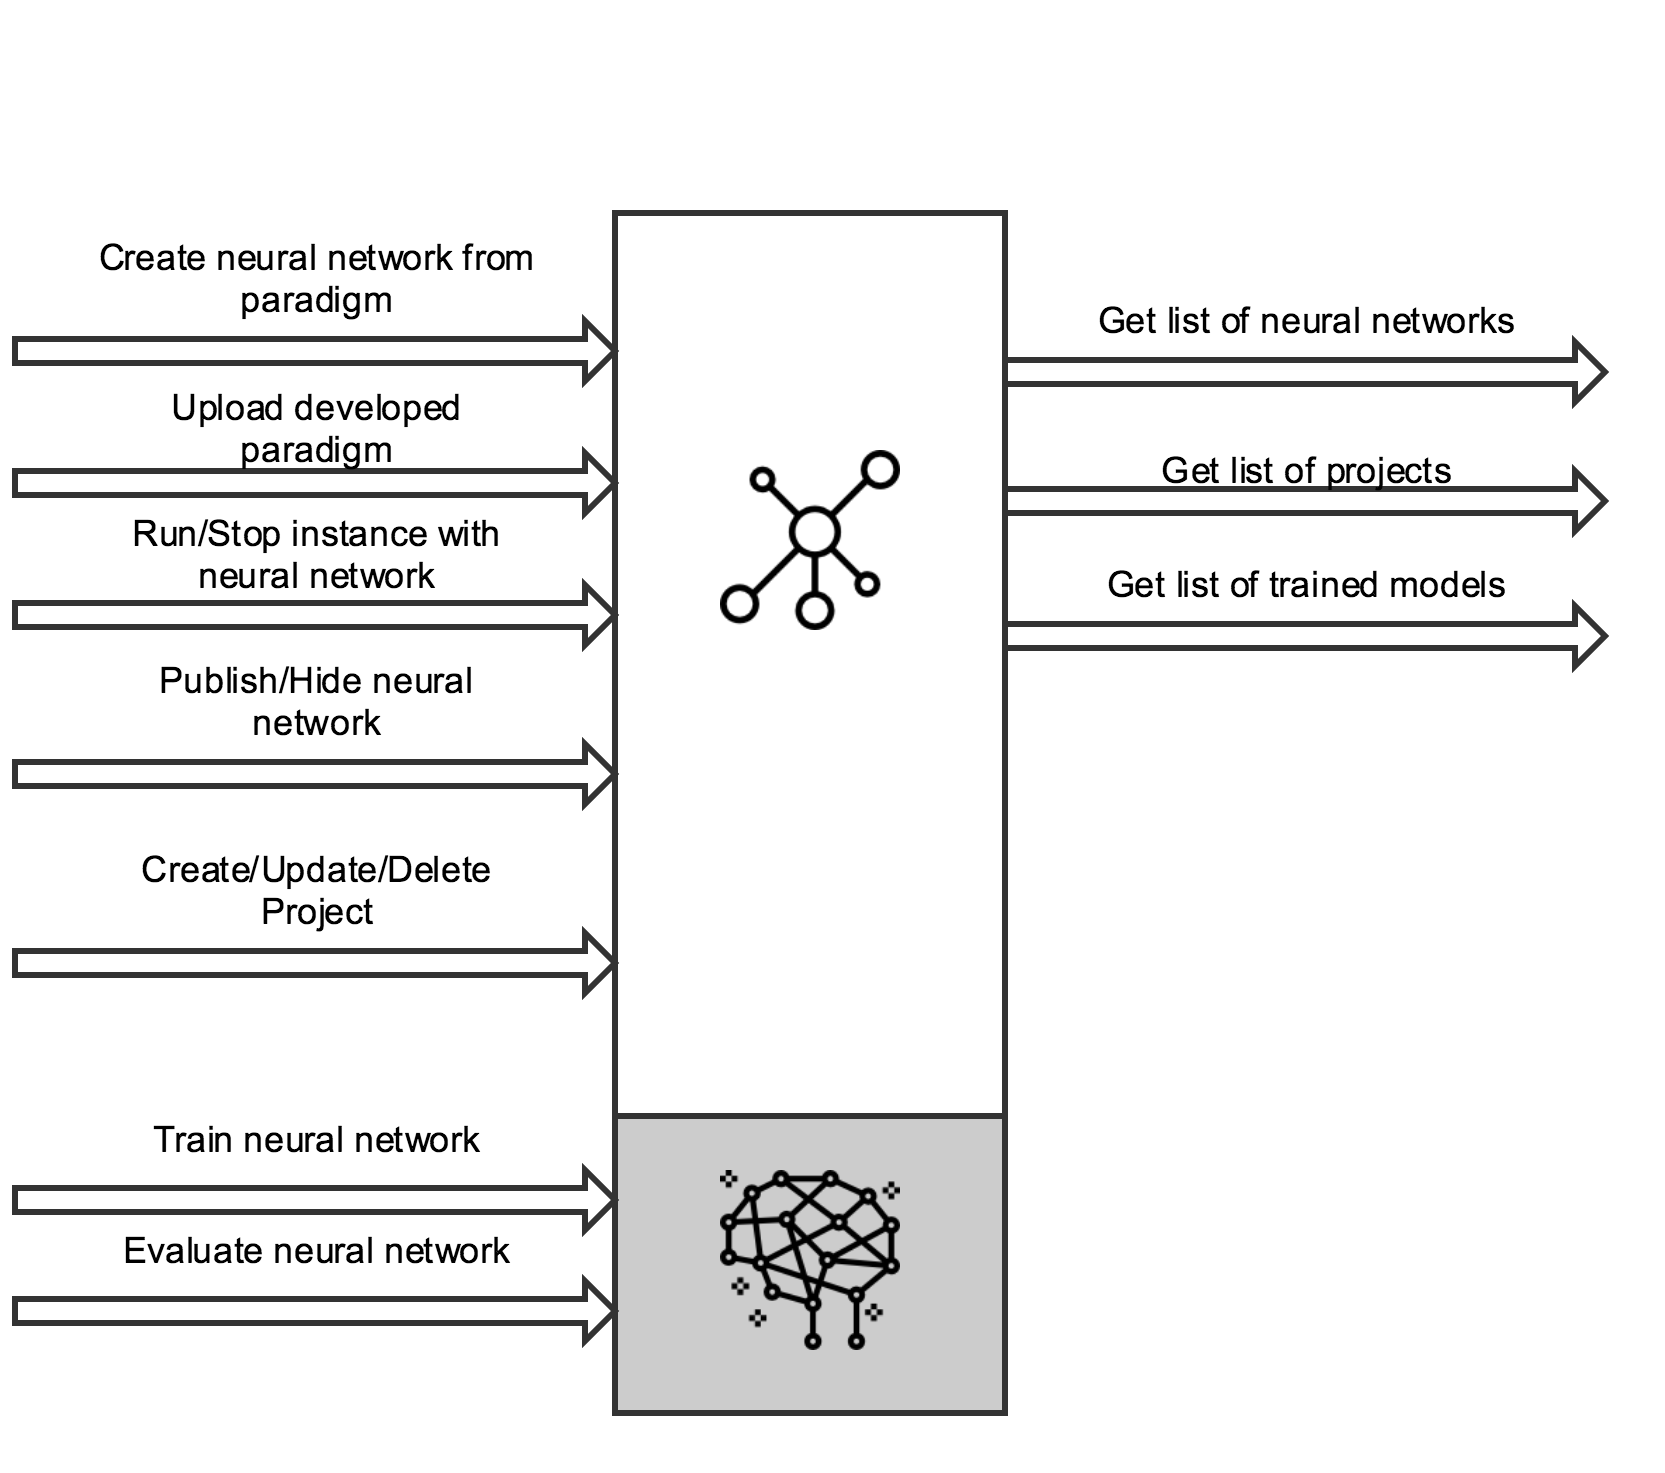
\includegraphics[width=\linewidth]{components/3/components/model_serivce.png}
  \caption{N2Sky Model Repository Web Service}
  \label{fig:model_serivce}
\end{center}
\end{figure}

As it is shown in figure \ref{fig:model_serivce} Model Repository Web Service has following accessible services:

\begin{itemize}
\item Create neural network from paradigm
\item Upload developed neural network paradigm
\item Run/Stop instance of neural network
\item Publish/Hide neural network 
\item Create/Update/Delete Project with neural networks
\item Get list of neural networks
\item Get list of projects
\item Get list of trained models 
\item Train neural network (accessible only for model management service itself)
\item Evaluate neural network (accessible only for model management service itself)
\end{itemize}

Detailed information about web service API and API documentation is written in \autoref{API Documentation}


There are two services embedded in the Model Repository web service and not exposed:

\begin{description}
\item[Training service.]  This service provides neural network training functionality. It is not possible to perform training to make the direct request on service endpoint. 

In order to perform training, the user has to know training input parameters and type of training file which can be accepted. This information is stored in ViNNSL schema. 
 
Only Model Repository web service can trigger this service after being insured that environment available and ready to perform tests. Training a is a long-term process, but it does not block an entire application. This service writes log data to the instance. Model Repository repository makes a callback to training service in order to check if training is completed. If training still processing, the Model Repository Service will fetch the log data in order to present current training result. The user can also decide to stop training process if he is satisfied with the current result.

If the user performs training on his own neural network he can also log result about his network and environment behavior. 
\item[Testing service.] The testing service allows users to evaluate a trained model.  Testing data is described in ViNNSL format. Normally testing is not a long-term process because it is running against trained neural network model. Since there is absolute freedom by neural network structure customization, the testing process can be inefficient and could take some resources from the environment. Considering this face it was decided to encapsulate this process too. 
\end{description}

\subsubsection{Cloud Management Web Service.}\label{Cloud management Web Service}  Cloud web service is originally available only for the system administrator. This service can manage OpenStack environment and Cloudify container management system. On every OpenStack instance as we as on OpenStack itself the monitoring management system service is installed. Every monitoring management system has its own metrics configurations and alerting rules. The monitoring service is only exposed via Cloud management web service. 
 
 Cloud management service supports Platform as a Service distribution. The system administrator can configure the service according to his needs. All rules, including configuration rules for monitoring and alert management systems, can be adjusted on demand.  
 
 
\begin{figure}[htbp]
\begin{center}
  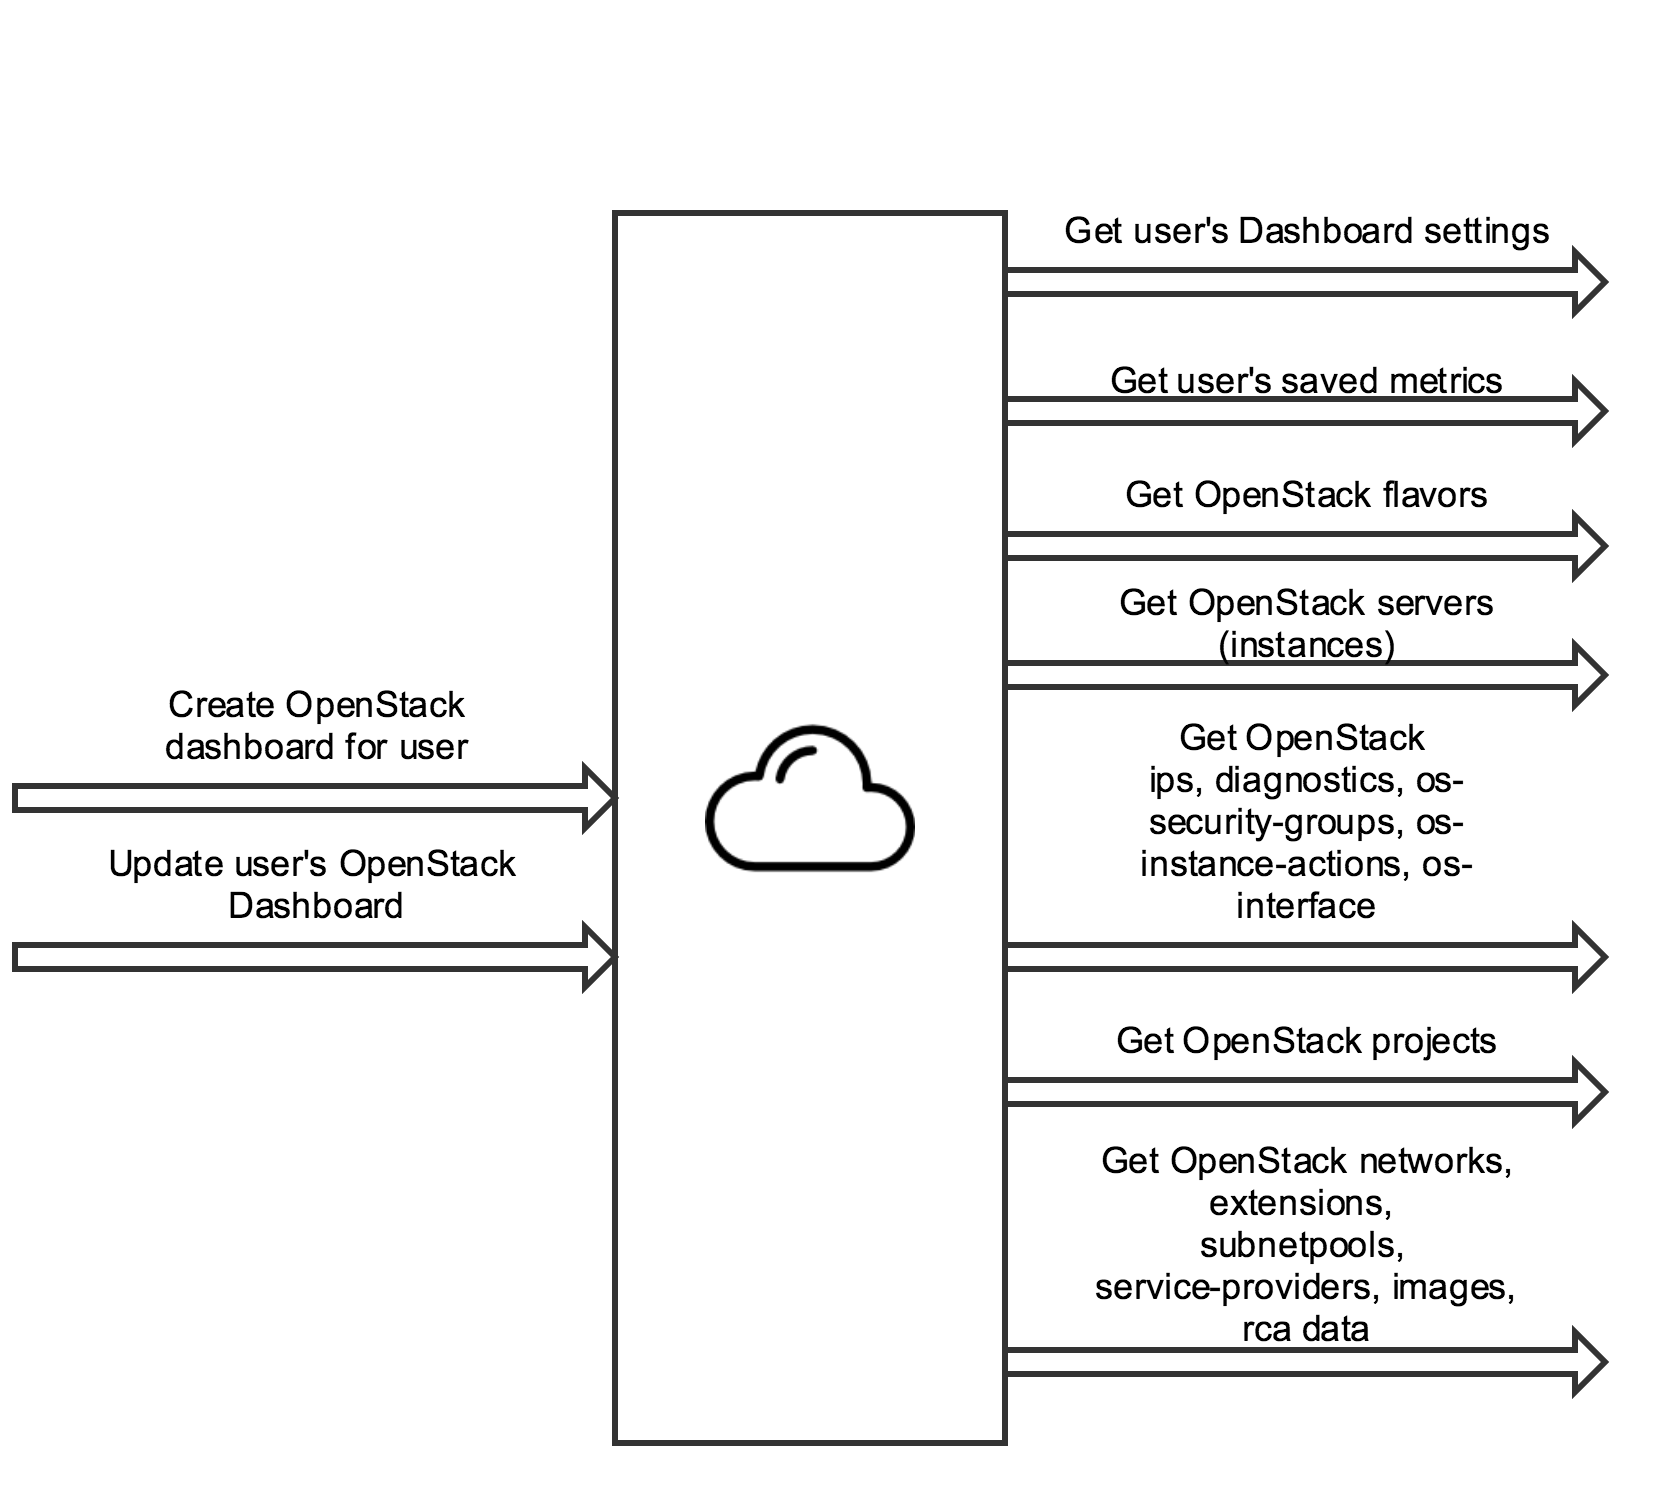
\includegraphics[width=\linewidth]{components/3/components/cloud_service.png}
  \caption{N2Sky Cloud Management Web Service}
  \label{fig:cloud_service}
\end{center}
\end{figure}

 
 As it is shown in figure \ref{fig:cloud_service} Cloud Management Web Service has following accessible services:

\begin{itemize}
\item Get user's Dashboard settings
\item Get user's saved metrics (reference to \autoref{Continuous Monitoring System} )
\item Get OpenStack Services: flavours, servers, networks, images etc.
\item Create / Update user's OpenStack Dashboard settings
\end{itemize}

Detailed information about web service API and API documentation is written in \autoref{API Documentation}


\subsection{Continuous Monitoring System}\label{Continuous Monitoring System}

In client-server architecture especially for OpenStack cloud platform, computer servers are important. Servers could go down, but the system-administrator does not have to work 24/7 in order to monitor the system and wait until some problem occurs. A system administrator could use some monitoring tools like Nagios for OpenStack in order to get information about servers state. Monitoring tool can give information about the system, network, and infrastructure \cite{nagios}. The purpose of the monitoring tool to find some problems and inform the system administrator about some problem occurred. This tool cannot solve the problem, but it can give information what went wrong.
 
\subsubsection{Monitoring requirements}\label{Monitoring requirements}

The base monitoring system is a readable and understandable representation of the graph. Graphs allow you to see objects beaning monitored and recognize metric from these objects. 
The good monitoring graph gives the meaningful description, helps quickly to detect and determine issues via representation. This kind of graph should serve as a motivation for action to solve problems. 
There are some simple rules, which makes graphing well:

\begin{description}
\item[Consistency.] Representation should correctly reflect reality. All objects, which are represented on the graph, must be correlated with a real data on the machine. 
\item[Graphs need to make sense.]  All lines represented on the chart have to be readable and understandable.  Fake or unreadable information could cause problems. Metrics set should be small, one metric represent one object. There is no need to put multiple objects which do not bind directly to one chart.
\item[Stacked area vs. multiline area.] Not every chart should have the same visual representation of the lines. Depending on the case we can decide which type of area to use.  If there are small time series with a high frequency it is better to use multiline area and stacked area on longer time series but with a bigger metric set respectively. 
\item[Understanding graph before starting to analyze it. ] Since there are going to be multiple charts with a different metrics we need to make sure that every user can understand the meaning of the particular graph. Good naming fulfilled contend and correct positioning is very important.
\item[Data hierarchy. ] It is important to define groups, metrics, data points and nested levels on the chart.  Groups help to bind similar objects together. Data points give information of time stamps. Metrics is actual graph representation. The nested level is multiple line metrics. All mentioned data should be visible and accessible. 
\item[Clarity.] Designing a chart it is important to take into consideration that there are multiple devices with a different screen resolution. Too many lines on limited space will make chart unreadable.  If there are lots of charts on one page it makes people confused what a meaning of this page. That is why it is a good practice to create multiple pages with grouped charts. 
\item[Perspective.] It is important to put graphs in such perspective so that any deviation will be easily noticeable. 
\item[Appeal.] All charts are people-oriented, people today like a simple and clean appearance of the applications and if an application has lots of charts they need to be with an appropriate design.  
\item[Control and managing.] It should be possible for any user to manipulate a graph. Either to change time series or remove some metric, customization of the graph makes the whole application more attractive.
\end{description}

\subsubsection{Applying Monitoring}\label{Applying Monitoring}
To build continues monitoring system there is a need to use a toolkit with an active ecosystem.  Searching for a proper toolkit the toolkit should be fulfilled some specific requirements that going to be used in N2Sky:
\begin{itemize}
\item Proper and self-describable metric name with a key pairs
\item Possibility to query metrics and join them in one graph.
\item Not resource-intensive
\item Support HTTP/HTTPS protocol
\item Collect and push to repository time series
\item Scalable
\end{itemize}

After researching it was decided to go for Prometheus Monitoring Toolkit \cite{alert_overview}. This tool support all requested requirements. One of the most interesting features is that Prometheus can be used on any UNIX environment. Since in OpenStack multiple instances with a different operating system can be created, Prometheus will match exact our needs. 
Originally Prometheus was created by SoundCloud team in 2012. The core of monitoring application is Prometheus server, which collects time series data from the moment it was executed on the environment as it is shown in figure \ref{fig:prometherus_arch}. All components are written in Go language and support multiple modules for monitoring different environment metrics. 
To understand the nature of Prometheus it is necessary to explain its architecture. 

\begin{figure}[htbp]
\begin{center}
  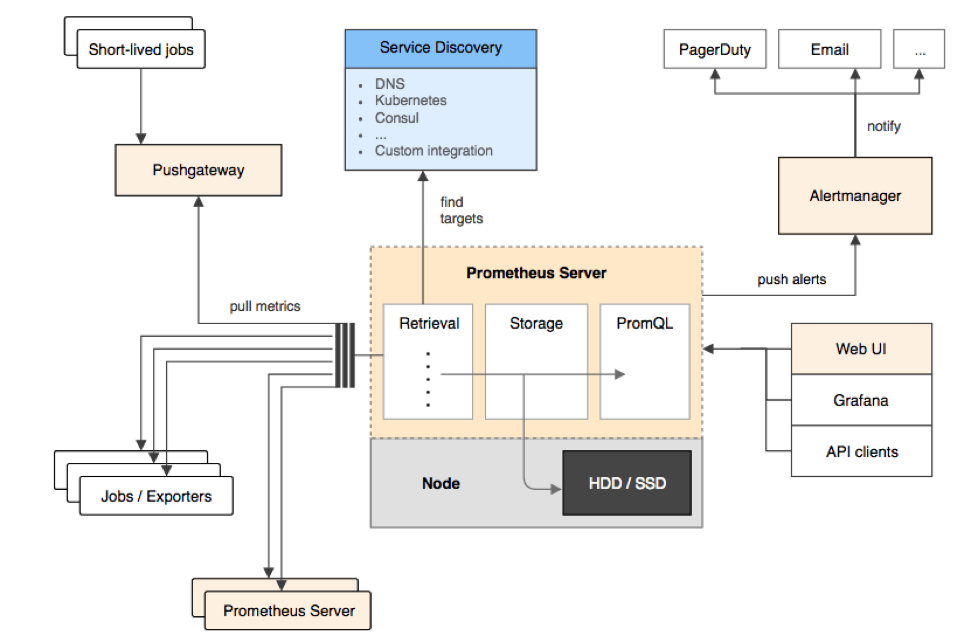
\includegraphics[width=\linewidth]{components/3/prometherus_arch.png}
  \caption{Prometheus monitoring architecture}
  \label{fig:prometherus_arch}
\end{center}
\end{figure}

The core Prometheus server pulls all metrics from jobs which are instrumented if the service is unavailable for instrumentation it can be pulled from push gateway. All metrics and logs data is stored locally so there is no distributed storage. It is possible to query this data to retrieve more specific information about particular metrics of joint metrics. N2Sky uses Prometheus API to build own customized dashboards. 
The common components of Prometheus architecture:
\begin{description}
\item[The Prometheus server.] This is the base element in the whole architecture. The server includes services which collection, storing and retrieving nodes. The principle is scrapping or pulling. It means that the data fetched with some interval, which can be configured and stored accordantly as a time series. Prometheus support different modules, each module represents some node. The nodes expose these ports that Prometheus uses for retrieving the data. For example, in N2Sky we are using Node Exporter Module which gives the possibility to collect almost all essential data like CPU, RAM, HDD/SSD etc.
\item[Push gateway.] There are some nodes, which are not exposing these endpoints. In this case collection of the data throw Push gateway is possible.  Prometheus short-lived jobs are executed to capture the data and convert it to the time series that can be used by Prometheus.
\item [Alert Manager.]  Monitoring consist of multiple metrics, each metric can be analyzed. It is possible to subscribe to particular metric in order to detect metric behavior namely metric deviations. Alert Management System used for firing events, it is possible to receive alert notification over multiple channels like Emails, SMS, Push notification etc.
\end{description}

Metric notation 
Following example represent metric notation:
\begin{lstlisting}
node_filesystem_avail {method="GET", endpoint="/api/posts", status="200"}
\end{lstlisting}

The metric naming is always self-described.  Requested metric "node\_filesystem\_avail" means available free space in the filesystem.  Every operating system has a different metric naming. N2Sky will propose the list of available metrics. In curly brackets defined the type of request, an endpoint and expected HTTP response status.

After executing this query the data will be retrieved from logs and represent as a time series as it is shown in figure \ref{fig:monitoring_req}.



\begin{figure}[htbp]
\begin{center}
  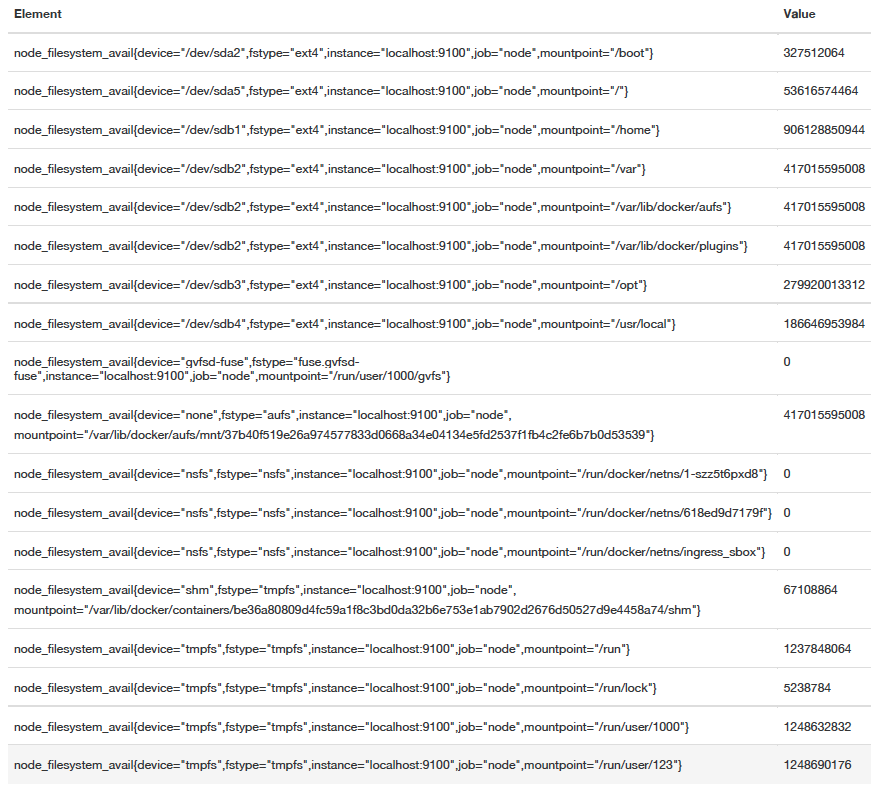
\includegraphics[width=\linewidth]{components/3/monitoring_req.png}
  \caption{Metric response}
  \label{fig:monitoring_req}
\end{center}
\end{figure}

One of the requirements of our monitoring system is scalability. One of the greatest features of Prometheus is that event if environment going to be overloaded it will generate the same amount of metrics anyway. Hence the amount of events is independent of the amount of generated time series. 
Talking about requirements it is important to mention here that there is a possibility to build joint metrics namely build multiple time series using this kind of metric:

\begin{description}
\item[Counter] The counter is a metric is representing a simple numerical value which can be incremented but not inverse. One of the typical examples is a number of expectations to have occurred. 
\item[Gauge] The gauge is a metric, which also represents a simple numerical value like a counter, but it is bidirectional. It means that this value can be decremented. The common example is CPU usage, which can go up and down.
\item[Histogram] The histogram is a metric, which represents observations.  It is stored in a bucket, which can be pulled. Any bucket can be configured depending on the need. It can be the sum of values or count of events, which are observed.
\item[Summary] The summary is a metric, which is similar to histogram but it calculates configurable quantities. 
\end{description}

\subsubsection{Integration with N2Sky}\label{Integration with N2Sky}

Prometheus supports query language, which is a key feature of this tool. The Prometheus query language, or promql, is expressive. 
With Prometheus, the self-described metric name can be chosen. Prometheus converts all metric so that every human can understand what exactly particular metric means. Let's take a previous example with a metric "node\_filesystem\_avail". This metric will show the folders on root and available memory on each of it.

\begin{lstlisting}
    node_filesystem_avail 
        {device="/dev/sdb4",fstype="ext4",
        instance="localhost:9100",job="node",
        ssmountpoint="/usr/local"}
\end{lstlisting}

Following request means that on "/usr/local" 186.6 GB is available. 

There is also the possibility to check a response code, which especially useful for alerting. 

\begin{lstlisting}
        node_filesystem_avail {status="500"}
\end{lstlisting}

This request returns some response code 500 namely internal server error. 

For building a proper dashboard for monitoring it is important to provide customization that is why Prometheus supports time duration:

\begin{itemize}
\item s - seconds
\item m - minutes
\item h - hours
\item d - days
\item w - weeks
\item y - years
\end{itemize}

Using the time duration with an offset it is possible to get an exact metric on demand. 
Building query with a Prometheus can bring lots of advantages. For example, there is the query which  a counter with an available node file system metric:

\begin{lstlisting}
    took( 3, sum(
         rate(api_http_requests_total{status=500}[1h]
    ) )
     by (endpoint)
     )
\end{lstlisting}

This query is already complicated, but it can be extended by multiple new rules and constraints. 

In N2Sky was developed monitoring service, which uses microservices approach like an entire application. It was decided to get rid of complex queries and provide some intuitive way of creating metrics. 
First of all the time range add a complexity. It was decided that the user should give only time interval and step. Let's say the user wants to see CPU load for the last hour with a step 30 seconds. It makes the creation of metric more intuitive, no more range like "from", "to" and type of ranges. All this can be solved with one simple request. 
The second part is a storing of metric. Instead of every time build a query the monitoring service saving requested by user metric. In this case, every user will get his own customized metric. 
The service uses Mongo DB for storing the metric configuration. Every collection has its own schema. When a user makes a request to save a metric the schema has to be filled with a requested by user data.

\subsubsection{Monitoring dashlet Design}\label{Monitoring dashlet Design}

Since there are multiple machine and services to monitor there was a need to create a dedicated dashboard design.  At first, let's take a look at the environments we have to monitor: 
\begin{description}
\item[Openstack Machine.]  It is dedicated machine, our cloud base for development and running instances.
\item[Openstack Instances.]   Virtual machines with a different OS.
\item[Docker Containers.]  Virtual machines in the OpenStack instances.
\end{description}

One of the most important parts of application design is to maximize reusability of the components. 


The benefit of the microservices architecture is the independence of each service. The good part of it, when one of the services will not be accessible, the rest of them still be up and running. The problem is that in order to make application running correctly all services are required. It is important to detect events and rollbacks the transaction in case if the error or failure occurs. N2Sky system has its own monitoring and alerting system, which notify the system administrator about failures, but how to handle events, which are transactionally dependent from service to service in case if the error occurs and an event is still in the transaction. There is two main kind of events \cite{cs5366}: 

\begin{itemize}
\item \emph{Intrinsic Events.} Process steps starting and finishing generate events intrinsic to the process model. This kind of events contains the process step or failure. 
\item \emph{Context Events.} Events stemming from the context of the process.
\end{itemize}

It is impossible to maintain each event and process an event stream in the N2Sky application because if some other developers forget to put the event into the stream it will not be noticed. That is why in N2Sky is events intrinsic, which are logging every transaction from one service to another. In case if the error occurs the alerting event will be fired with a log data like the step it self and the error. 

 
\begin{figure}[htbp]
\begin{center}
  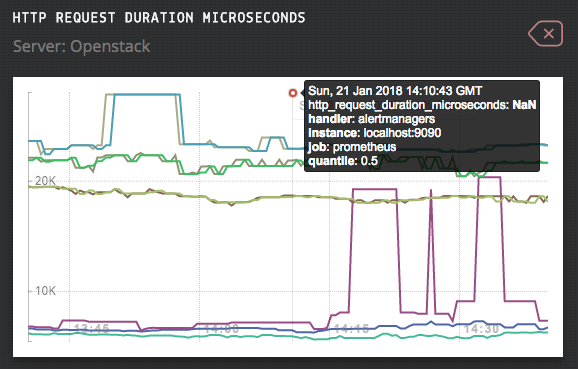
\includegraphics[scale=0.65]{components/3/components/monitoring_dashlet.png}
  \caption{N2Sky Monitoring Dashlet}
  \label{fig:monitoring_dashlet}
\end{center}
\end{figure}

 
The figure \ref{fig:monitoring_dashlet}  shows HTTP request directions in milliseconds metrics. Each dashlet item contains:
\begin{itemize}
\item Title, which represents readable and self-described metric name.
\item Server, which shows to which instance this metric belongs.
\item Chart is the monitoring data itself. 
\item Tooltip, which appears on metric mouse over. Tooltip shows following data:
\begin{itemize}
\item Date of the particular position.
\item Name of metric
\item Instance environment 
\item Handler is an alert manager listener (reference to \autoref{Alerting Management System})
\item Cron job
\item Quintile 
\end{itemize}

\end{itemize}


\subsection{Alerting Management System}\label{Alerting Management System}

Today the most trending subject in monitoring area is a prediction and automated detection. It makes people free from 24/7 managing, maintaining, and monitoring system.
For monitoring, we are using Prometheus tool. Since this tool saving constantly logs data about the system it is possible to reuse this logs to build an alert system. 
Prometheus tool provides an Alert Manager module. Natively this tool supports different notification methods like email notification or some request on Slack. 

\subsubsection{Alerting System Architecture}\label{Alerting System Architecture}

Since the Alert Manager is a part of Prometheus Tool it has its own binary. The idea behind is to have only one Alert Manager and have monitoring tool on multiple machines. If the machine goes down or even Prometheus itself, the Alert Manager can catch and deliver this event. 
To understand how Alert Manager works it is essential to understand the architecture of the whole system as it is displayed in figure \ref{fig:alert_arch}.

\begin{figure}[htbp]
\begin{center}
  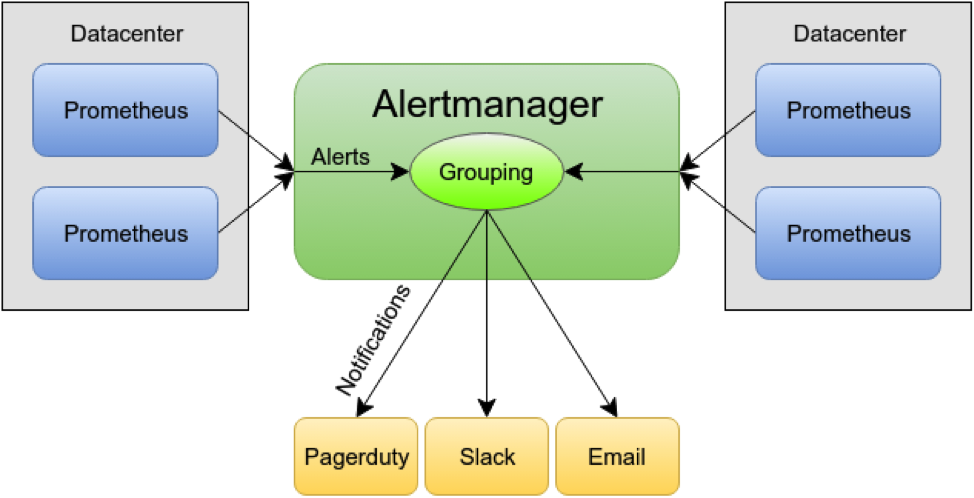
\includegraphics[scale=0.6]{components/3/alert_arch.png}
  \caption{Alerting System Architecture}
  \label{fig:alert_arch}
\end{center}
\end{figure}

This architecture is a typical messaging platform.
Messaging Service sends messages to multiple clients. It is implemented Producer-Consumer Pattern. In the Alert Manager Architecture, the role of the producer is taken by Prometheus Datacenter. Alert Manager consumes the messages. The consumer knows nothing about the producer and just subscribe to the event. With this approach, it is possible to attach multiple producers \cite{alert_book}. 

Alerts can be collected in groups by the datacenter. It means if an event occurs on multiple machines it can be packed into one notification and fired accordingly. 
In Prometheus configuration need to be set up only two things: reference on Alert Manager and Alert Rules. When Alert Manager consumes an event it just dispatches it via notification as it is displayed in figure \ref{fig:alert_arch_detailed}.

\begin{figure}[H]
\begin{center}
  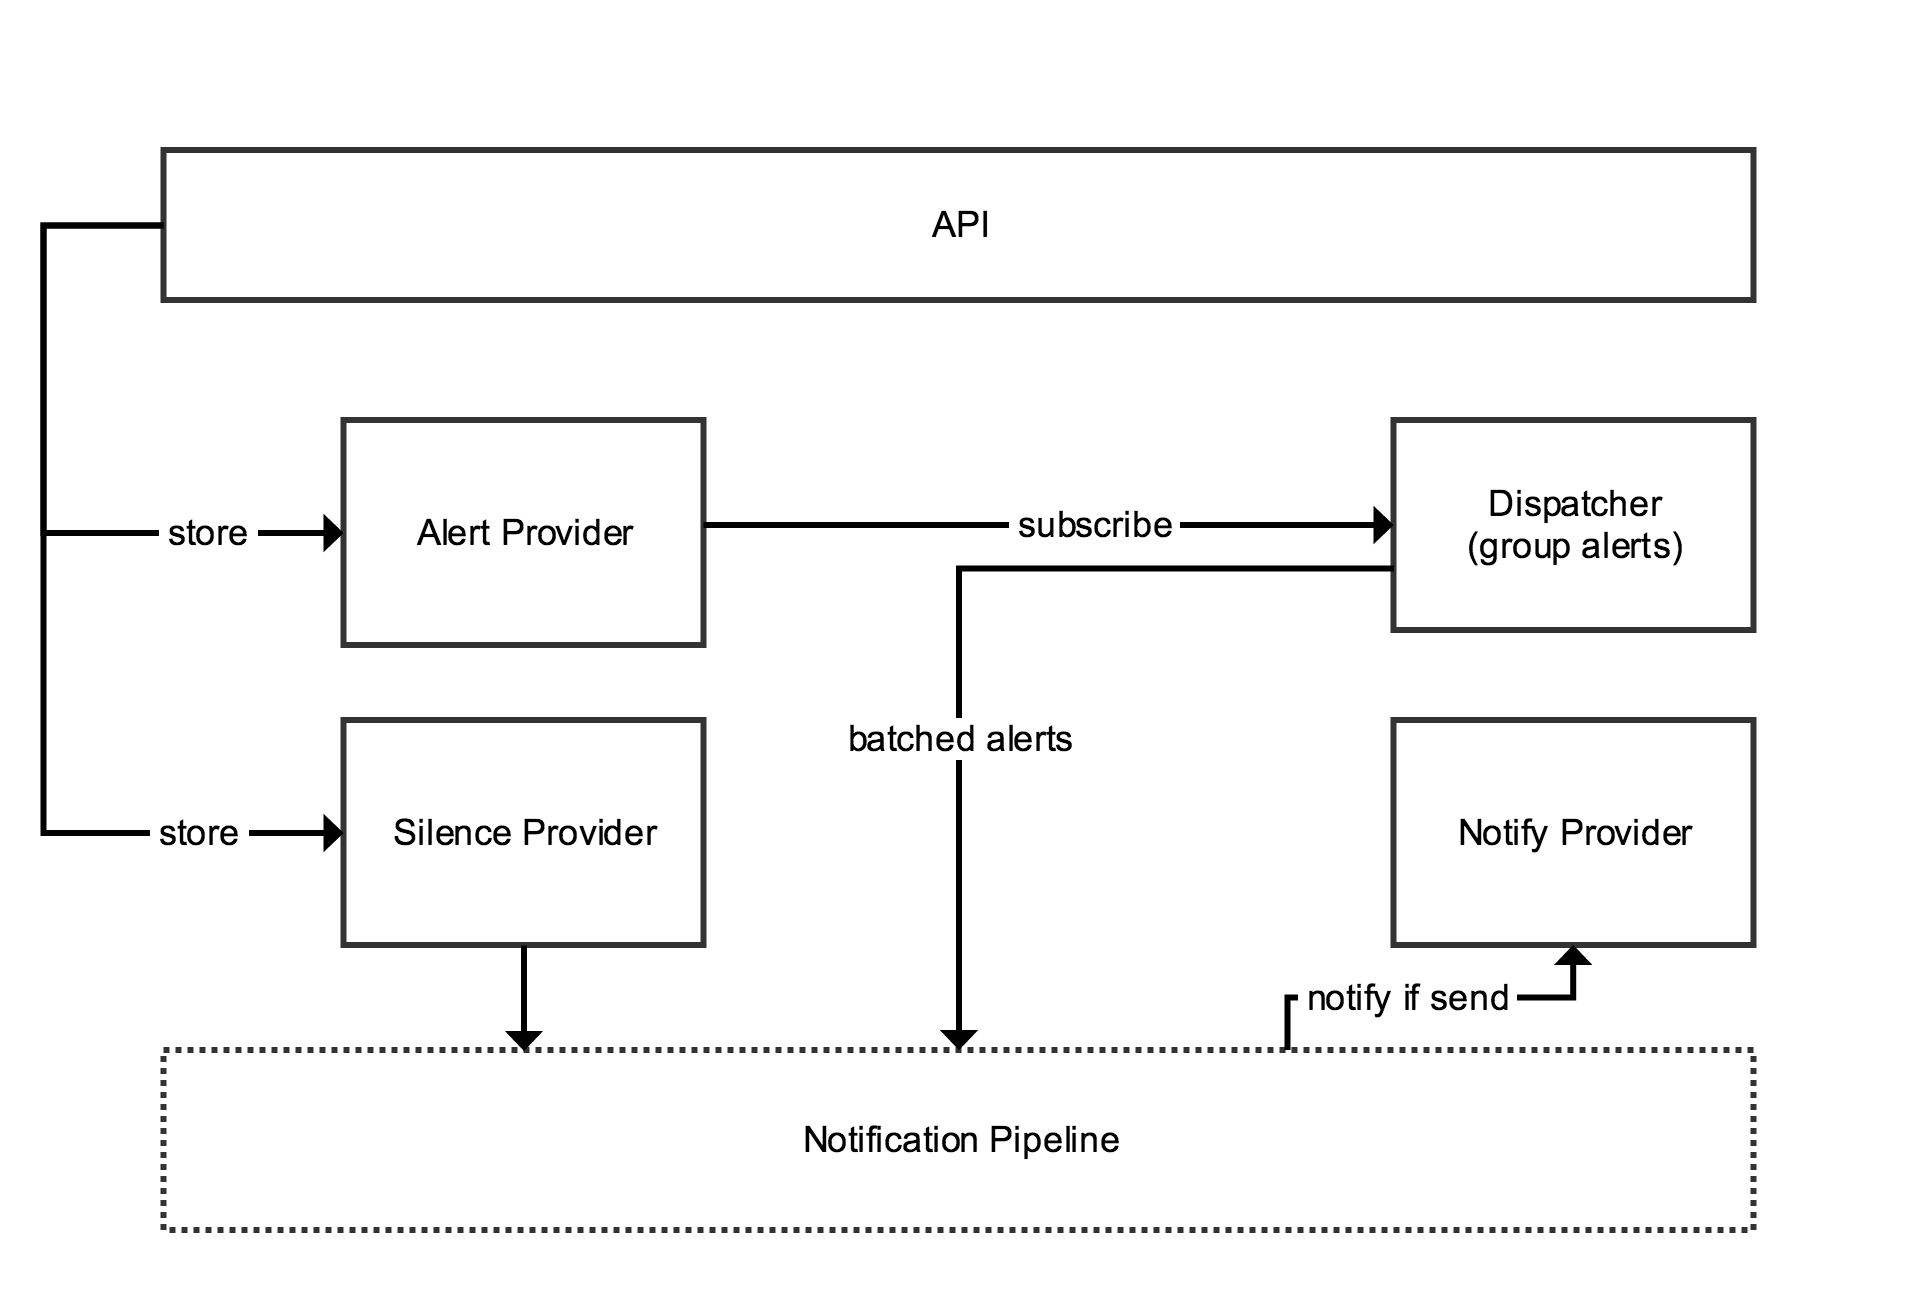
\includegraphics[width=\linewidth]{components/3/alert_details.png}
  \caption{Communication within Alerting Management System}
  \label{fig:alert_arch_detailed}
\end{center}
\end{figure}

\begin{description}
\item[API] Alert manager API has only one endpoint, which gives the list of events that occurred.
\begin{lstlisting}
            /api/v1/alerts
\end{lstlisting}

As a response the event information is sent \cite{alert_send}.
 \begin{lstlisting}
 [
  {
    "labels": {
      "<label>": "<value>"
    },
    "annotations": {
      "<label>": "<value>",
    },
    "startsAt": "<date>",
    "endsAt": "<date>"
    "generatorURL": "<url>"
  }
]
\end{lstlisting}
Following response shows timestamp of event, additional information as an annotation and name of event (alert). 
\item[Silences.] Silences is a commands, which are muting alerts for specific time. It can be configured via web interface. 
\item[Dispatcher.] Dispatcher is a grouping of alert with a similar nature into single notification. This will be send as a batch to Notification pipeline.
\item[Notification Pipeline.] Is a pipepline, which consists channel, router and filter. It takes rules from Alert Provider and Silence Provider and alerts from Dispatcher. If notification is ready it can be send. 
\end{description}


\subsubsection{Alert Rules}\label{Alert Rules}

As it was mention one of the main changes in Prometheus setup is to configure the alert rules. Every Prometheus Monitoring Tool can have it own alerting rules, which can be defined. There is also a possibility to reference on some common alerting rule for every monitoring system on every machine. 

 \begin{lstlisting}
        groups:
        - name: test
          rules:
          - alert: Error
            expr: job:request_latency_seconds:mean5m
            {job="loclhost:5000"} > 0.5
            for: 5m
            labels:
              severity: page
            annotations:
              summary: latency
\end{lstlisting}

Following the example of alerting rules shows the typical alerting rule. Most important parts are an expression, which is applied to Monitoring System and severity level.  More details about the creation of alerting rules are located in Development Guide chapter "Setting up Alert Management System" \autoref{Setting up Alert Management System}.

Alerting rules are instructions to the monitoring system it can be useful as well for alerting as for recording. 

Recording rules allow to pre-compute frequently needed expressions or expressions, which are resource or time-consuming.  These rules are saving the result in a new set of time series. It is like indexing this data, so that prevent expansive I/O methods. 
The rules are being executed sequentially with a predefined interval. 
With an alerting rule, it is possible to define alert namely deviation by particular expression from Prometheus Tool and its exports (modules). It allows building an alert even on the combined query. 

In case if Alert Manager is not available all alerts are saving into the buffer. As soon Alert Manager online all events will be fired sequentially. 



\subsubsection{Integration with N2Sky}\label{Integration with N2Sky Alerting}

Alerting System is represented as a module in N2Sky. 
Alerting Client is the additional configuration of Prometheus Monitoring System. When Prometheus will be executed it should have the reference to Alerting System and its rules. 
Since the client should be installed on each OpenStack instance it was integrated into image snapshot. When the new instance will be spawned with an OpenStack snapshot, the client will be automatically executed there.  

Alerting Client fire alerts depending on configured rules. The rules can be created via the user interface. The list of events N2Sky receives via its service, which fetches information from Alert System. 
 
\subsubsection{Alerting System Design}\label{Alerting System Design}

Developing Alerting System UI it kept the same design as in entire application. The N2Sky UI components were reused and none of the new components were created. The main component is a grid item which contains information about event, which is occurred  as it is shown in figure \ref{fig:alert_grid}.

\begin{figure}[htbp]
\begin{center}
  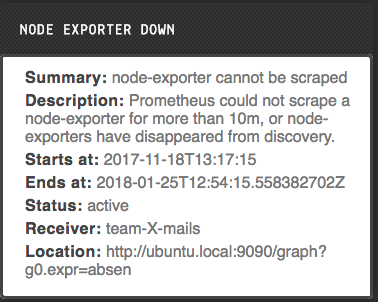
\includegraphics[scale=0.7]{components/3/alerts/alert_grid.png}
  \caption{N2Sky Alerting Management System Event representation.}
  \label{fig:alert_grid}
\end{center}
\end{figure}

The following information is shown:

\begin{description}
\item[Title.] The name of alert.
\item[Summary.]   Short is a description of the alert. If the summary is too long it will be cut.
\item[Description.] The whole description of the alert.
\item[Starts at.] Timestamp when the event occurred. 
\item[Ends at.] Timestamp when the event is no more valid. If the timestamp is a current day and time, the problem still not fixed. 
\item[Status.] Actual status of the event. Can be active and inactive.
\item[Receiver.] The group of receivers. Normally group contains multiple receivers emails. 
\item[Location.] The endpoint of the server where monitoring system installed. 
\end{description}

Every alert has its severity level. Depending on it the fired events will be represented differently. Every severity level has own color on N2Sky as it shown in ``Fig.~\ref{fig:alert_severity}''.

\begin{figure}[htbp]
\begin{center}
  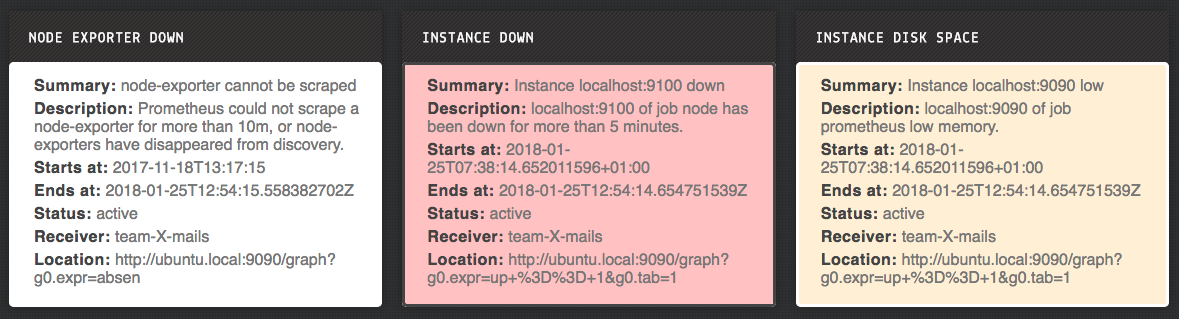
\includegraphics[width=\linewidth]{components/3/alerts/alert_severity.png}
  \caption{N2Sky Alerting Management System Severity Level}
  \label{fig:alert_severity}
\end{center}
\end{figure}

There are three types of severity levels:
\begin{itemize}
\item Critical, which shows that crucial event occurs. For example, if the server goes down it is critical severity level.  In N2Sky UI it has a red color. 
\item Warning, which shows that something goes wrong. For example not enough disk space on the server. In N2Sky UI it has the orange color. 
\item Page, which shows that some information. For example, lots of requests occurred. In N2Sky UI it has the white color.  
\end{itemize}
 



